\subsection{Implementation}

The implementation reads an RGB JPEG image and converts the RGB matrix
to a YCbCr representation. The $Y$ component is then retained as the
grayscale intensity matrix. From this grayscale matrix, three different
reference strategies are tested: a fixed reference of $128$, a global
mean reference, and Gaussian local references with two different values of $\sigma$ .\newline
The purpose of taking two differet scenarios is to clearly illustrate that the mode of clustering and averaging chosen depends on the type of image. For Example images with simple graphic arts prefer gaussian but those with complex graphics or natural photos work well with the global average referencing.\newline
Hence we have to use some machone learning algorithms and models so they can be trained with the data available about best referencing based on the situation, which will be used by them further for a new situation, and this implementation is beyond the scope of this article.
\vspace*{\baselineskip}
\subsection{Testing Case 1: Scenery}

The first test case uses a scenery image. The outputs are presented in
the following order so that the effect of each reference method can be
compared with the original image.

\begin{figure}[H]
    \centering
    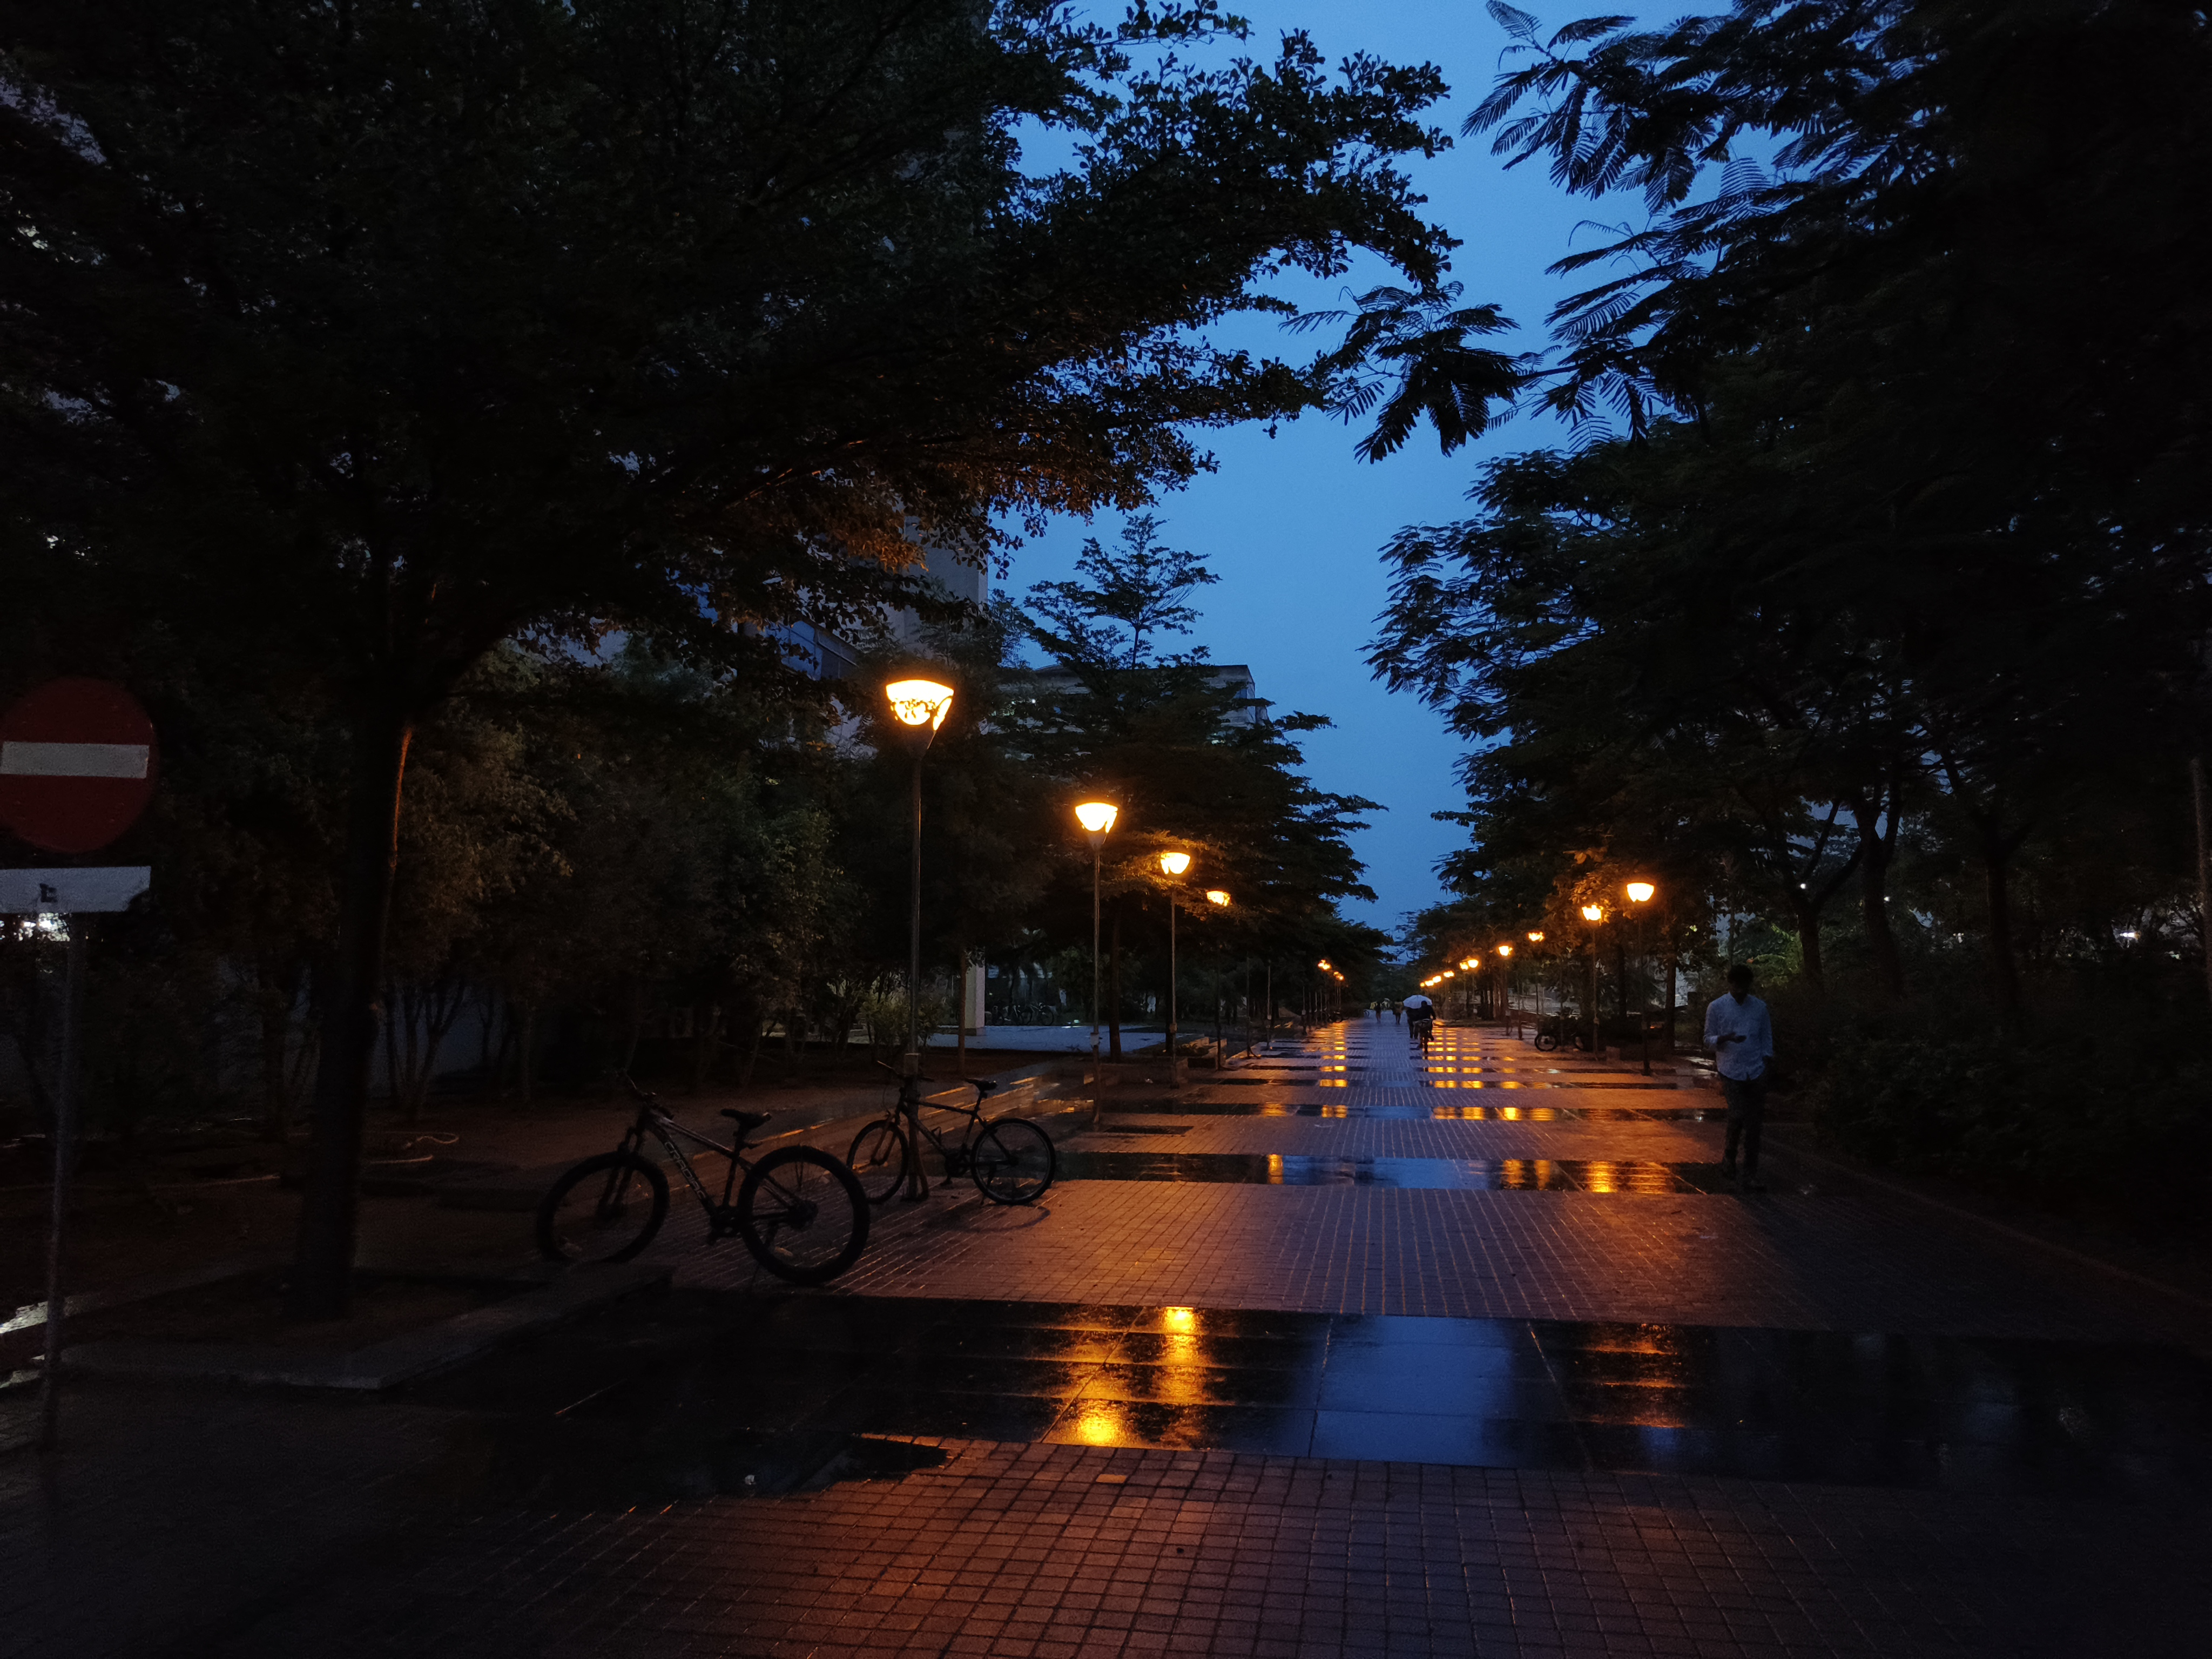
\includegraphics[width=0.5\linewidth]{figs/scenery/input.jpg}
    \caption{Input scenery image.}
    \label{fig:scenery_input}
\end{figure}

\begin{figure}[H]
    \centering
    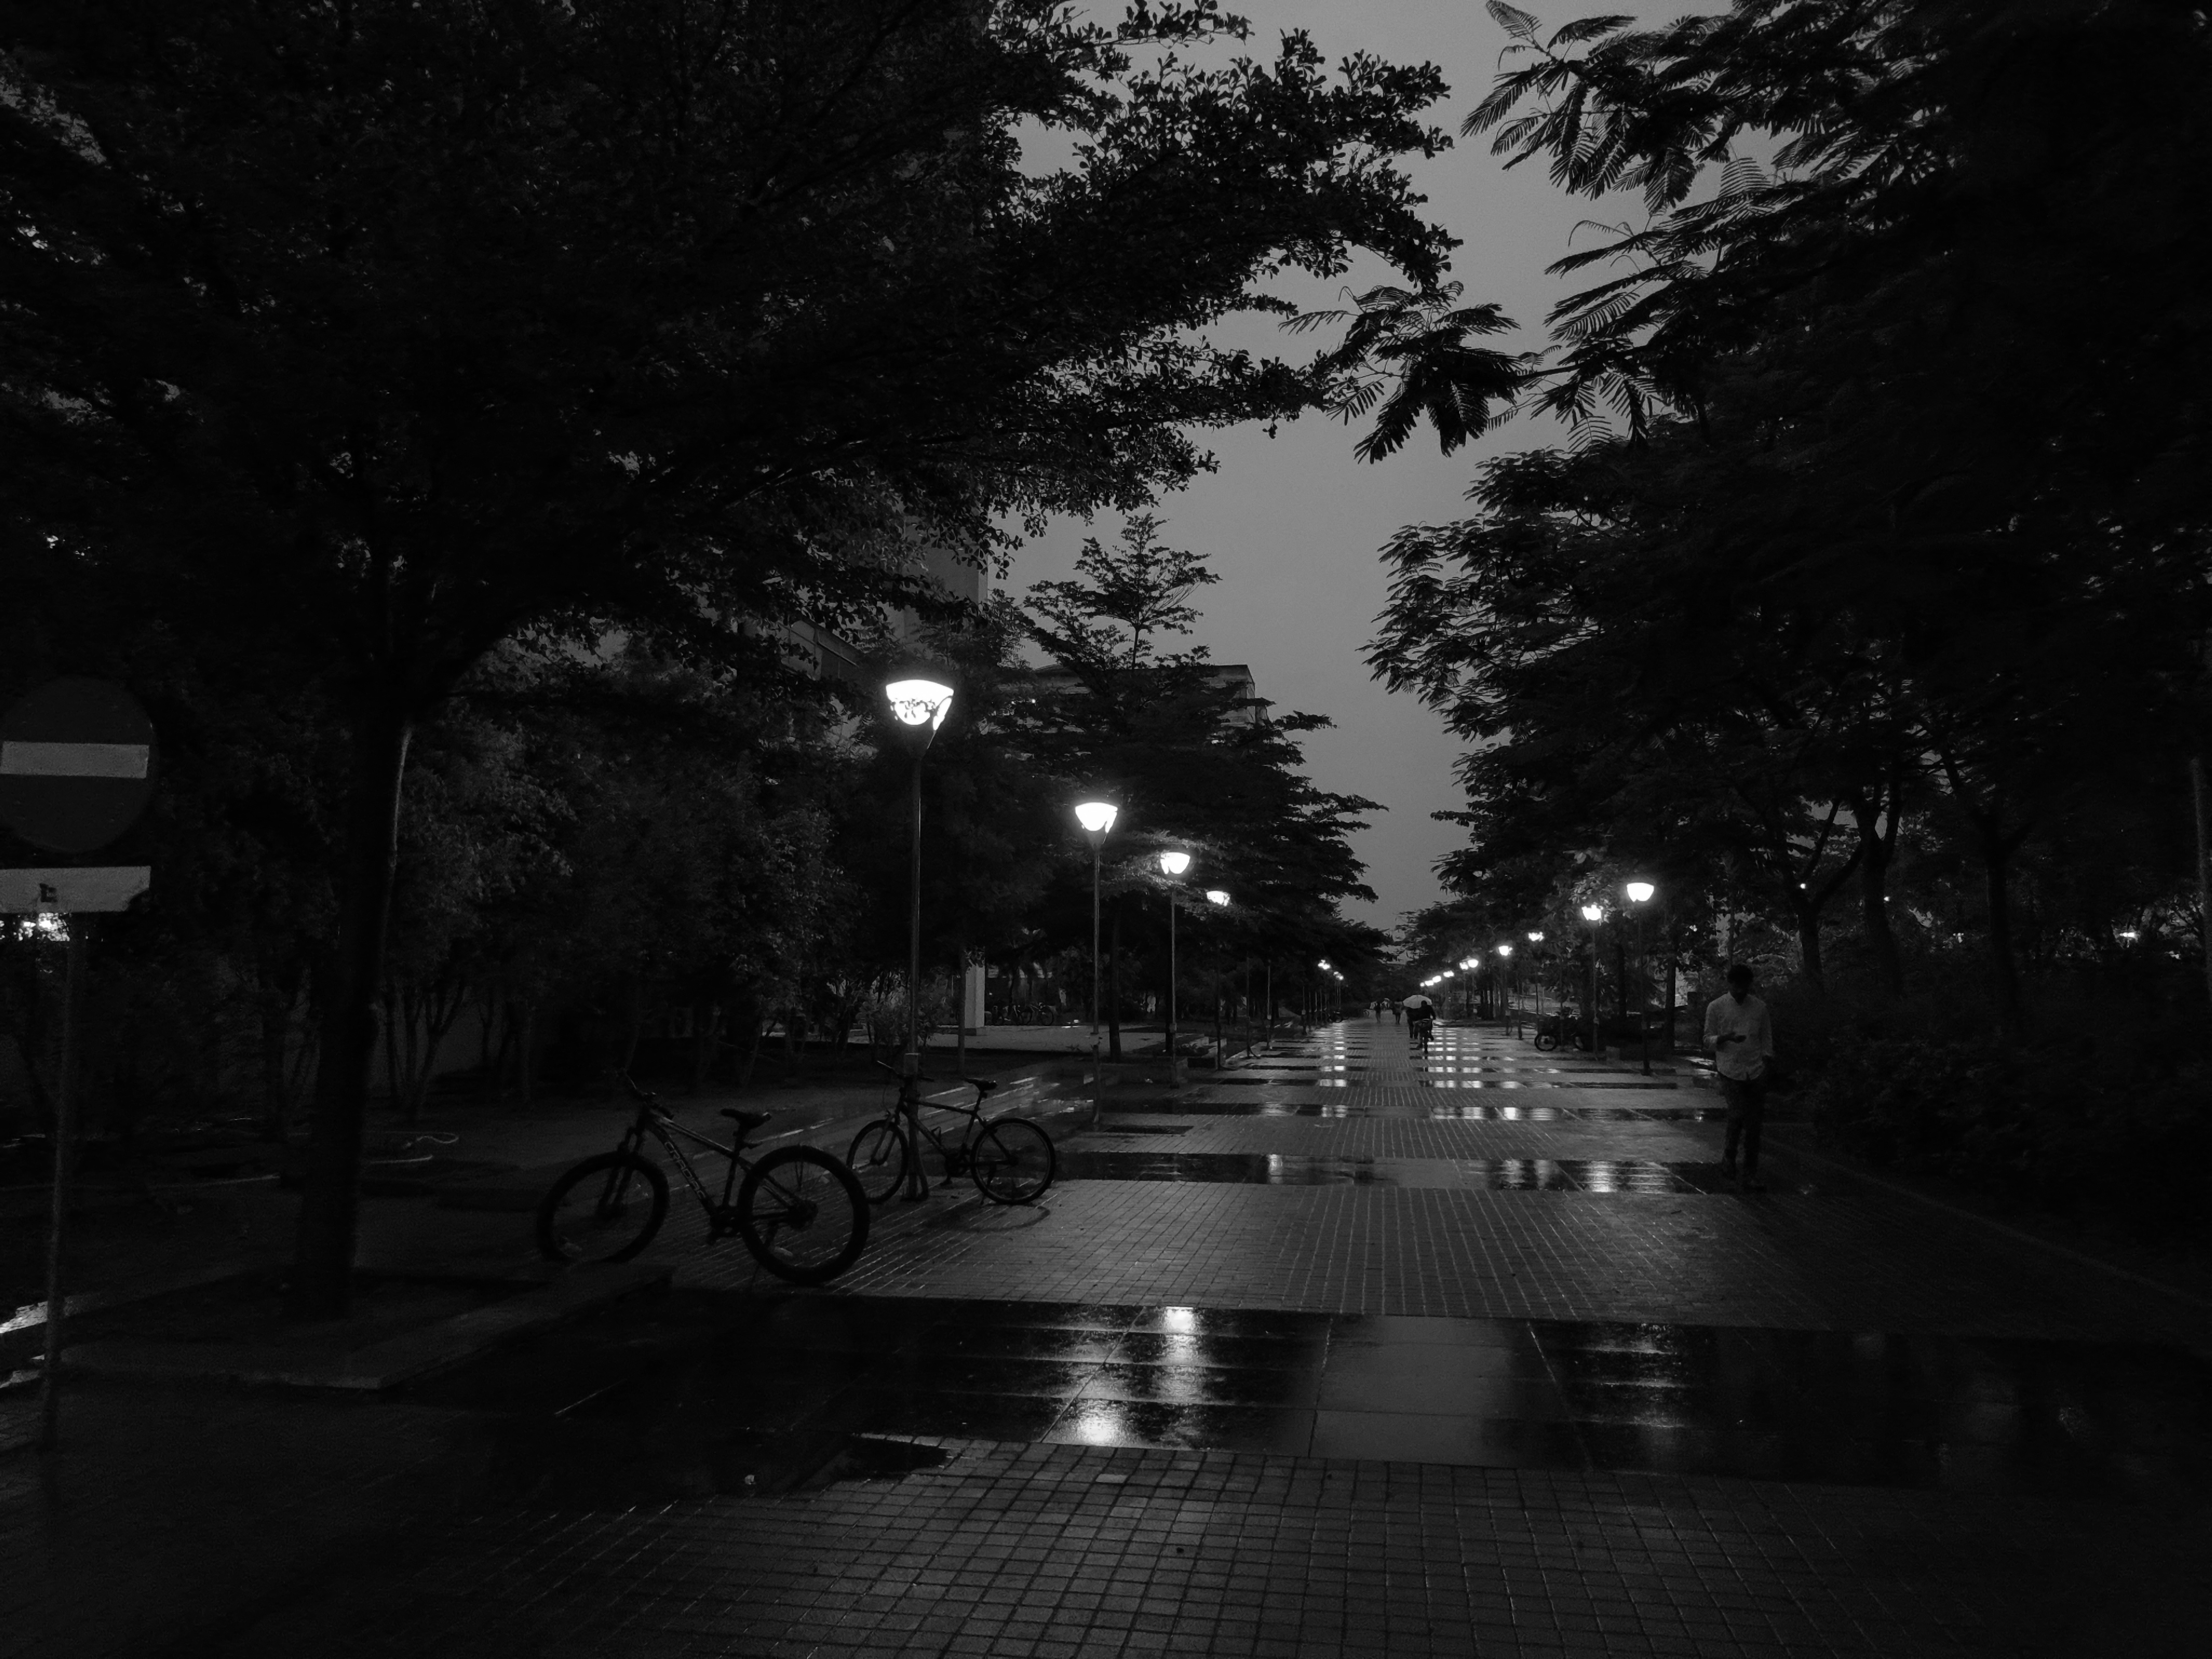
\includegraphics[width=0.5\linewidth]{figs/scenery/output_grayscale.pdf}
    \caption{Grayscale representation of the scenery image.}
    \label{fig:scenery_grayscale}
\end{figure}

\begin{figure}[H]
    \centering
    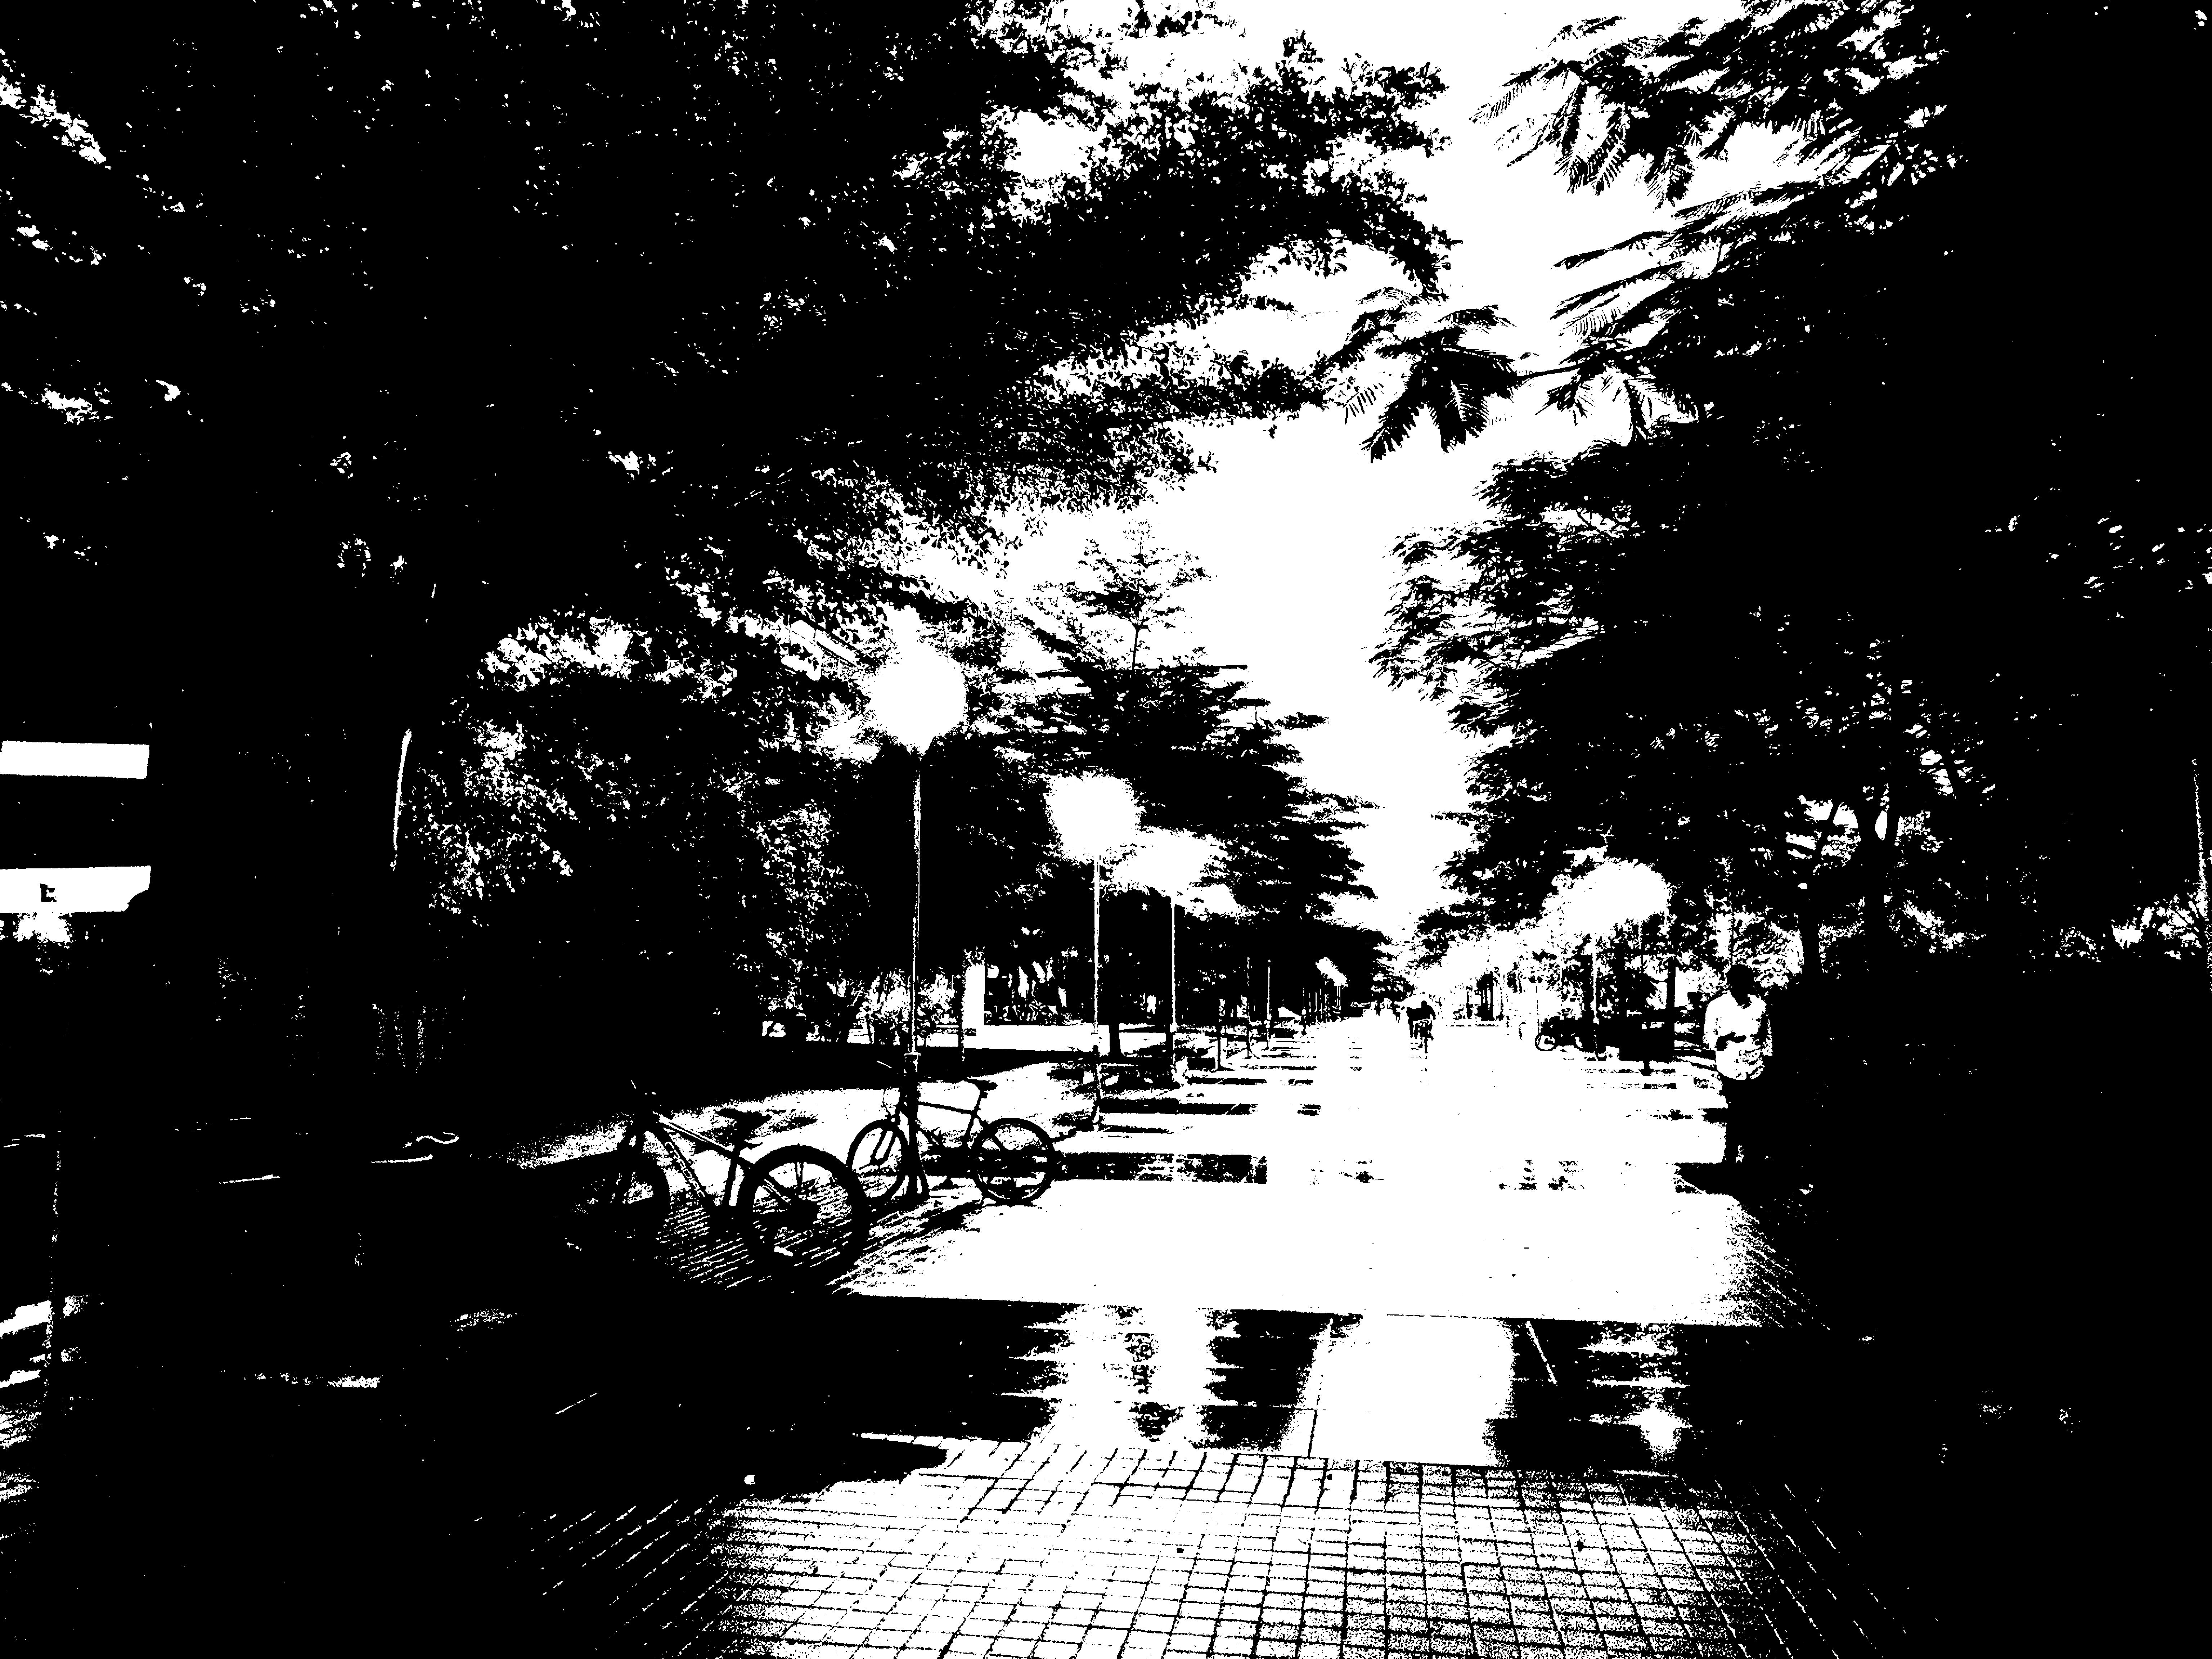
\includegraphics[width=0.5\linewidth]{figs/scenery/averaged_reference.pdf}
    \caption{Global mean adaptive thresholding of the scenery image.}
    \label{fig:scenery_adaptive}
\end{figure}

\begin{figure}[H]
    \centering
    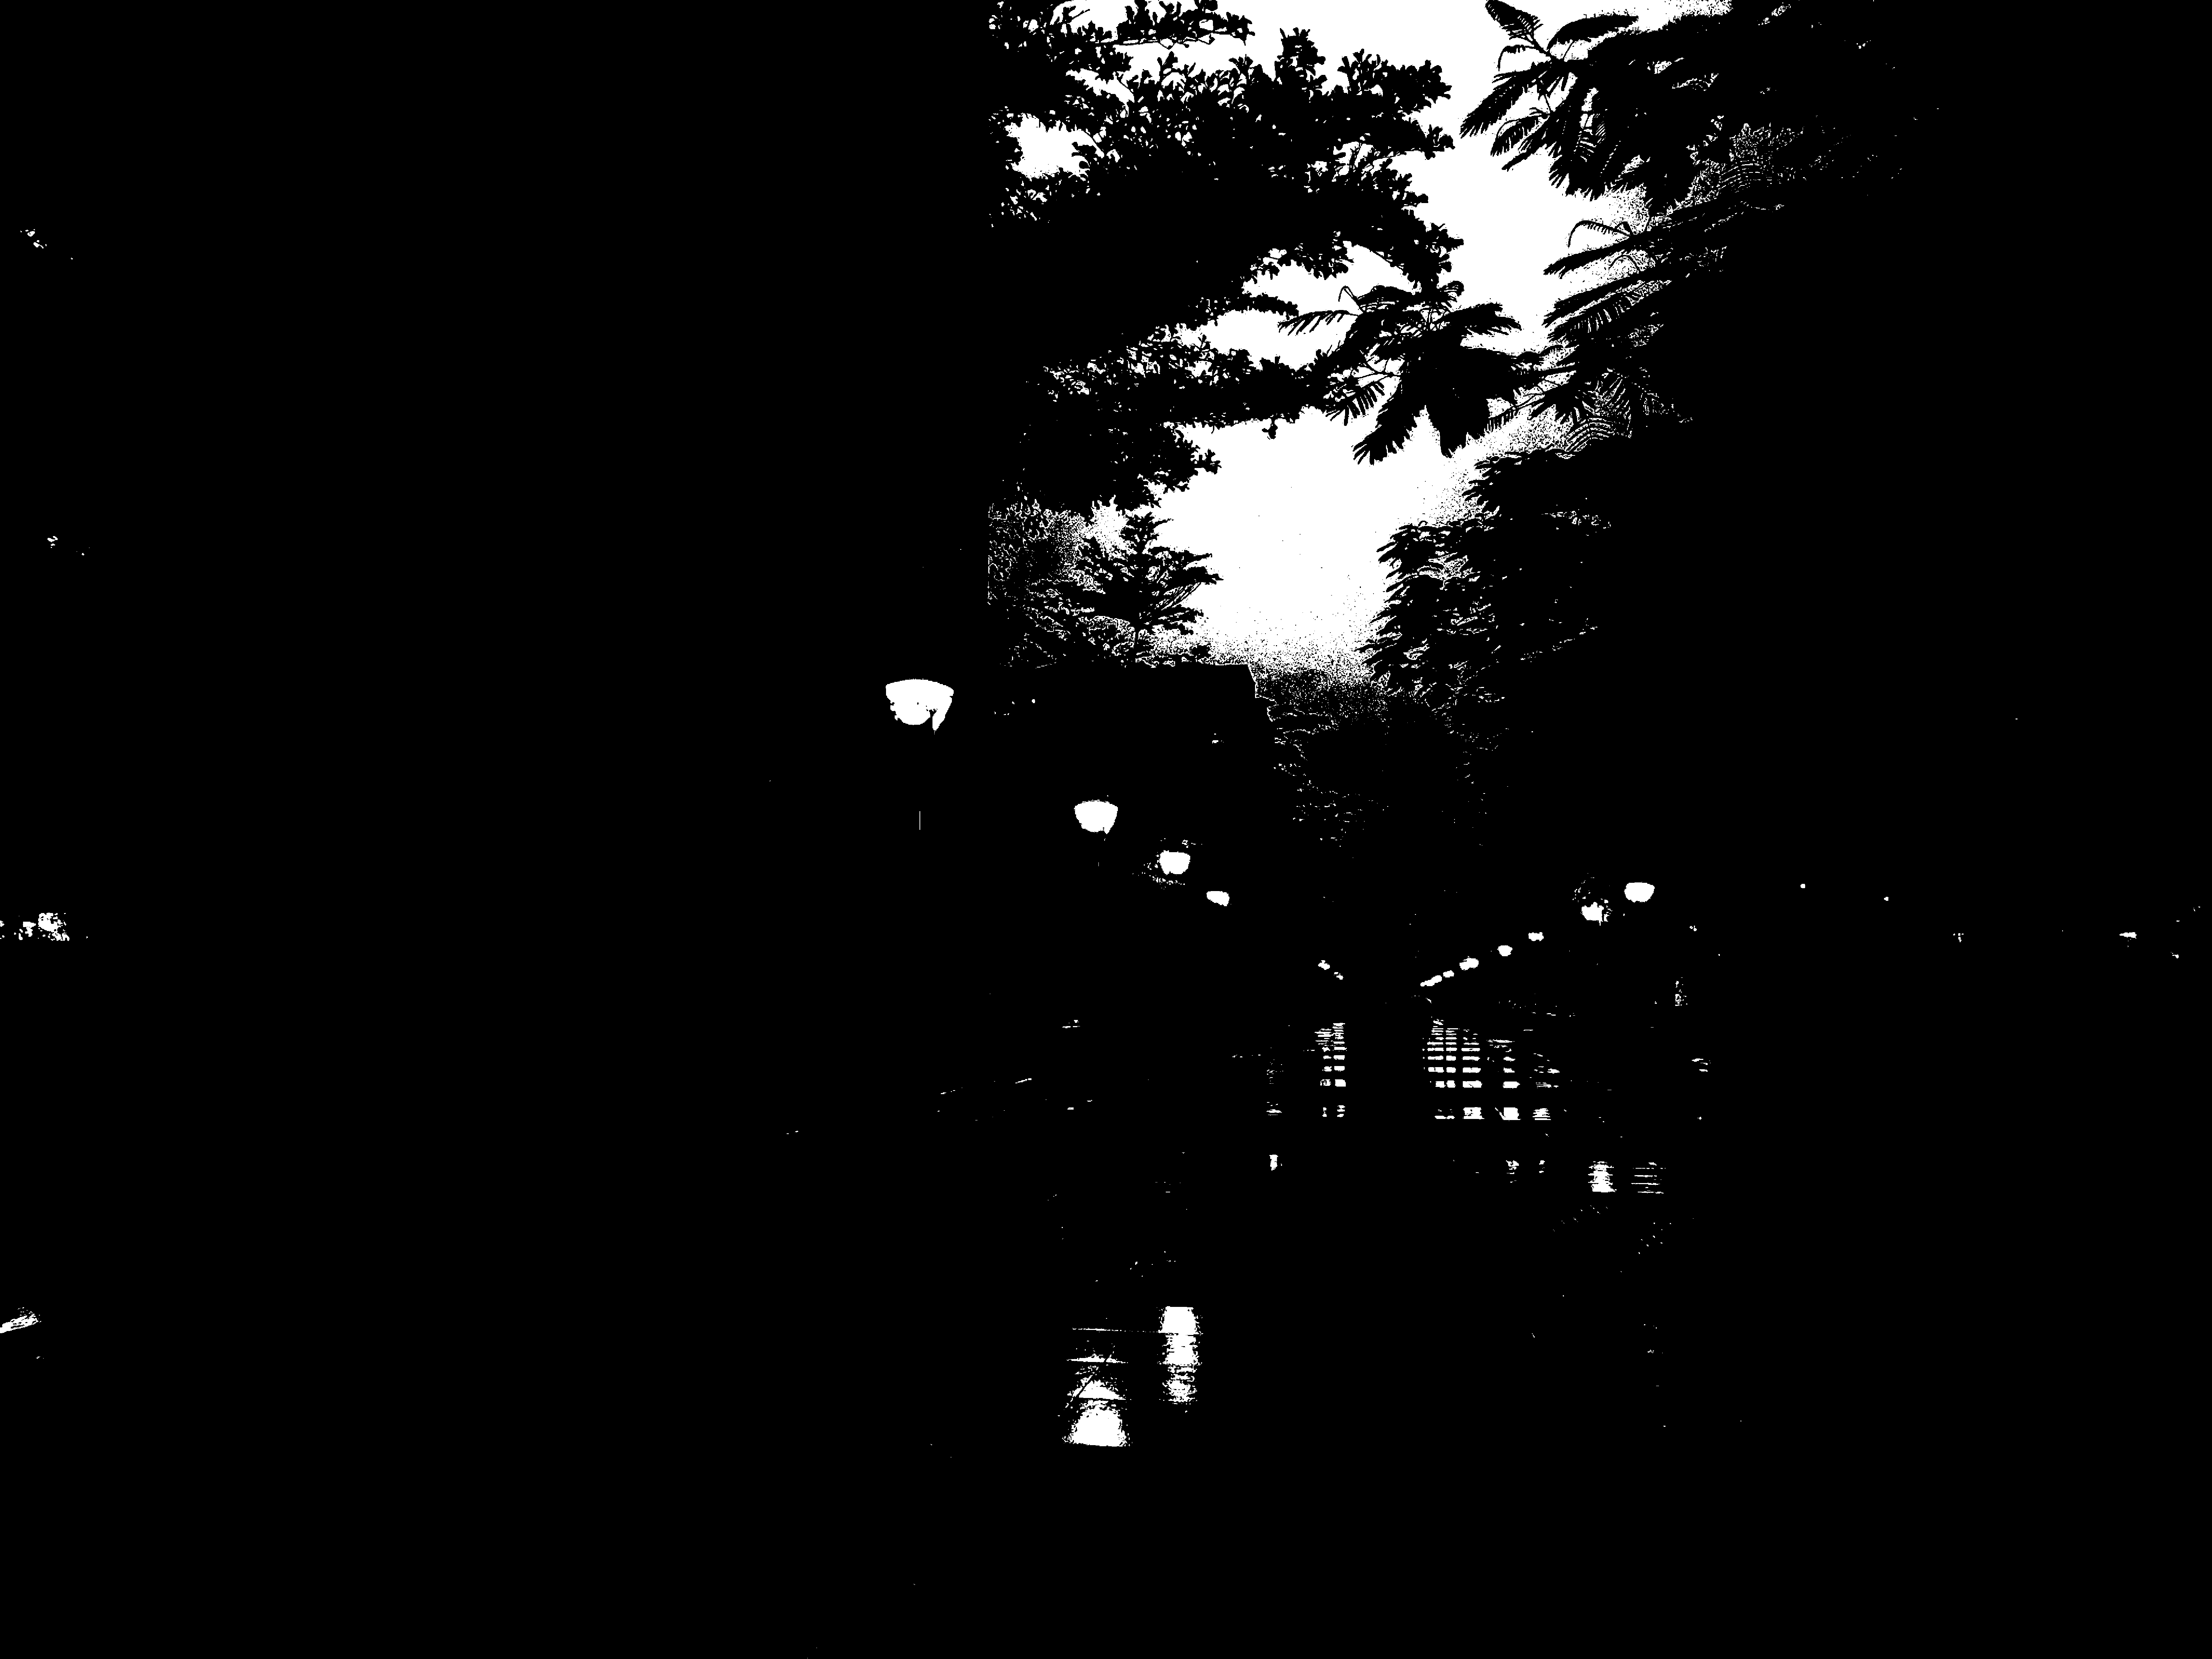
\includegraphics[width=0.5\linewidth]{figs/scenery/fixed_reference.pdf}
    \caption{Static thresholding using the fixed reference of $128$.}
    \label{fig:scenery_static}
\end{figure}

\begin{figure}[H]
    \centering
    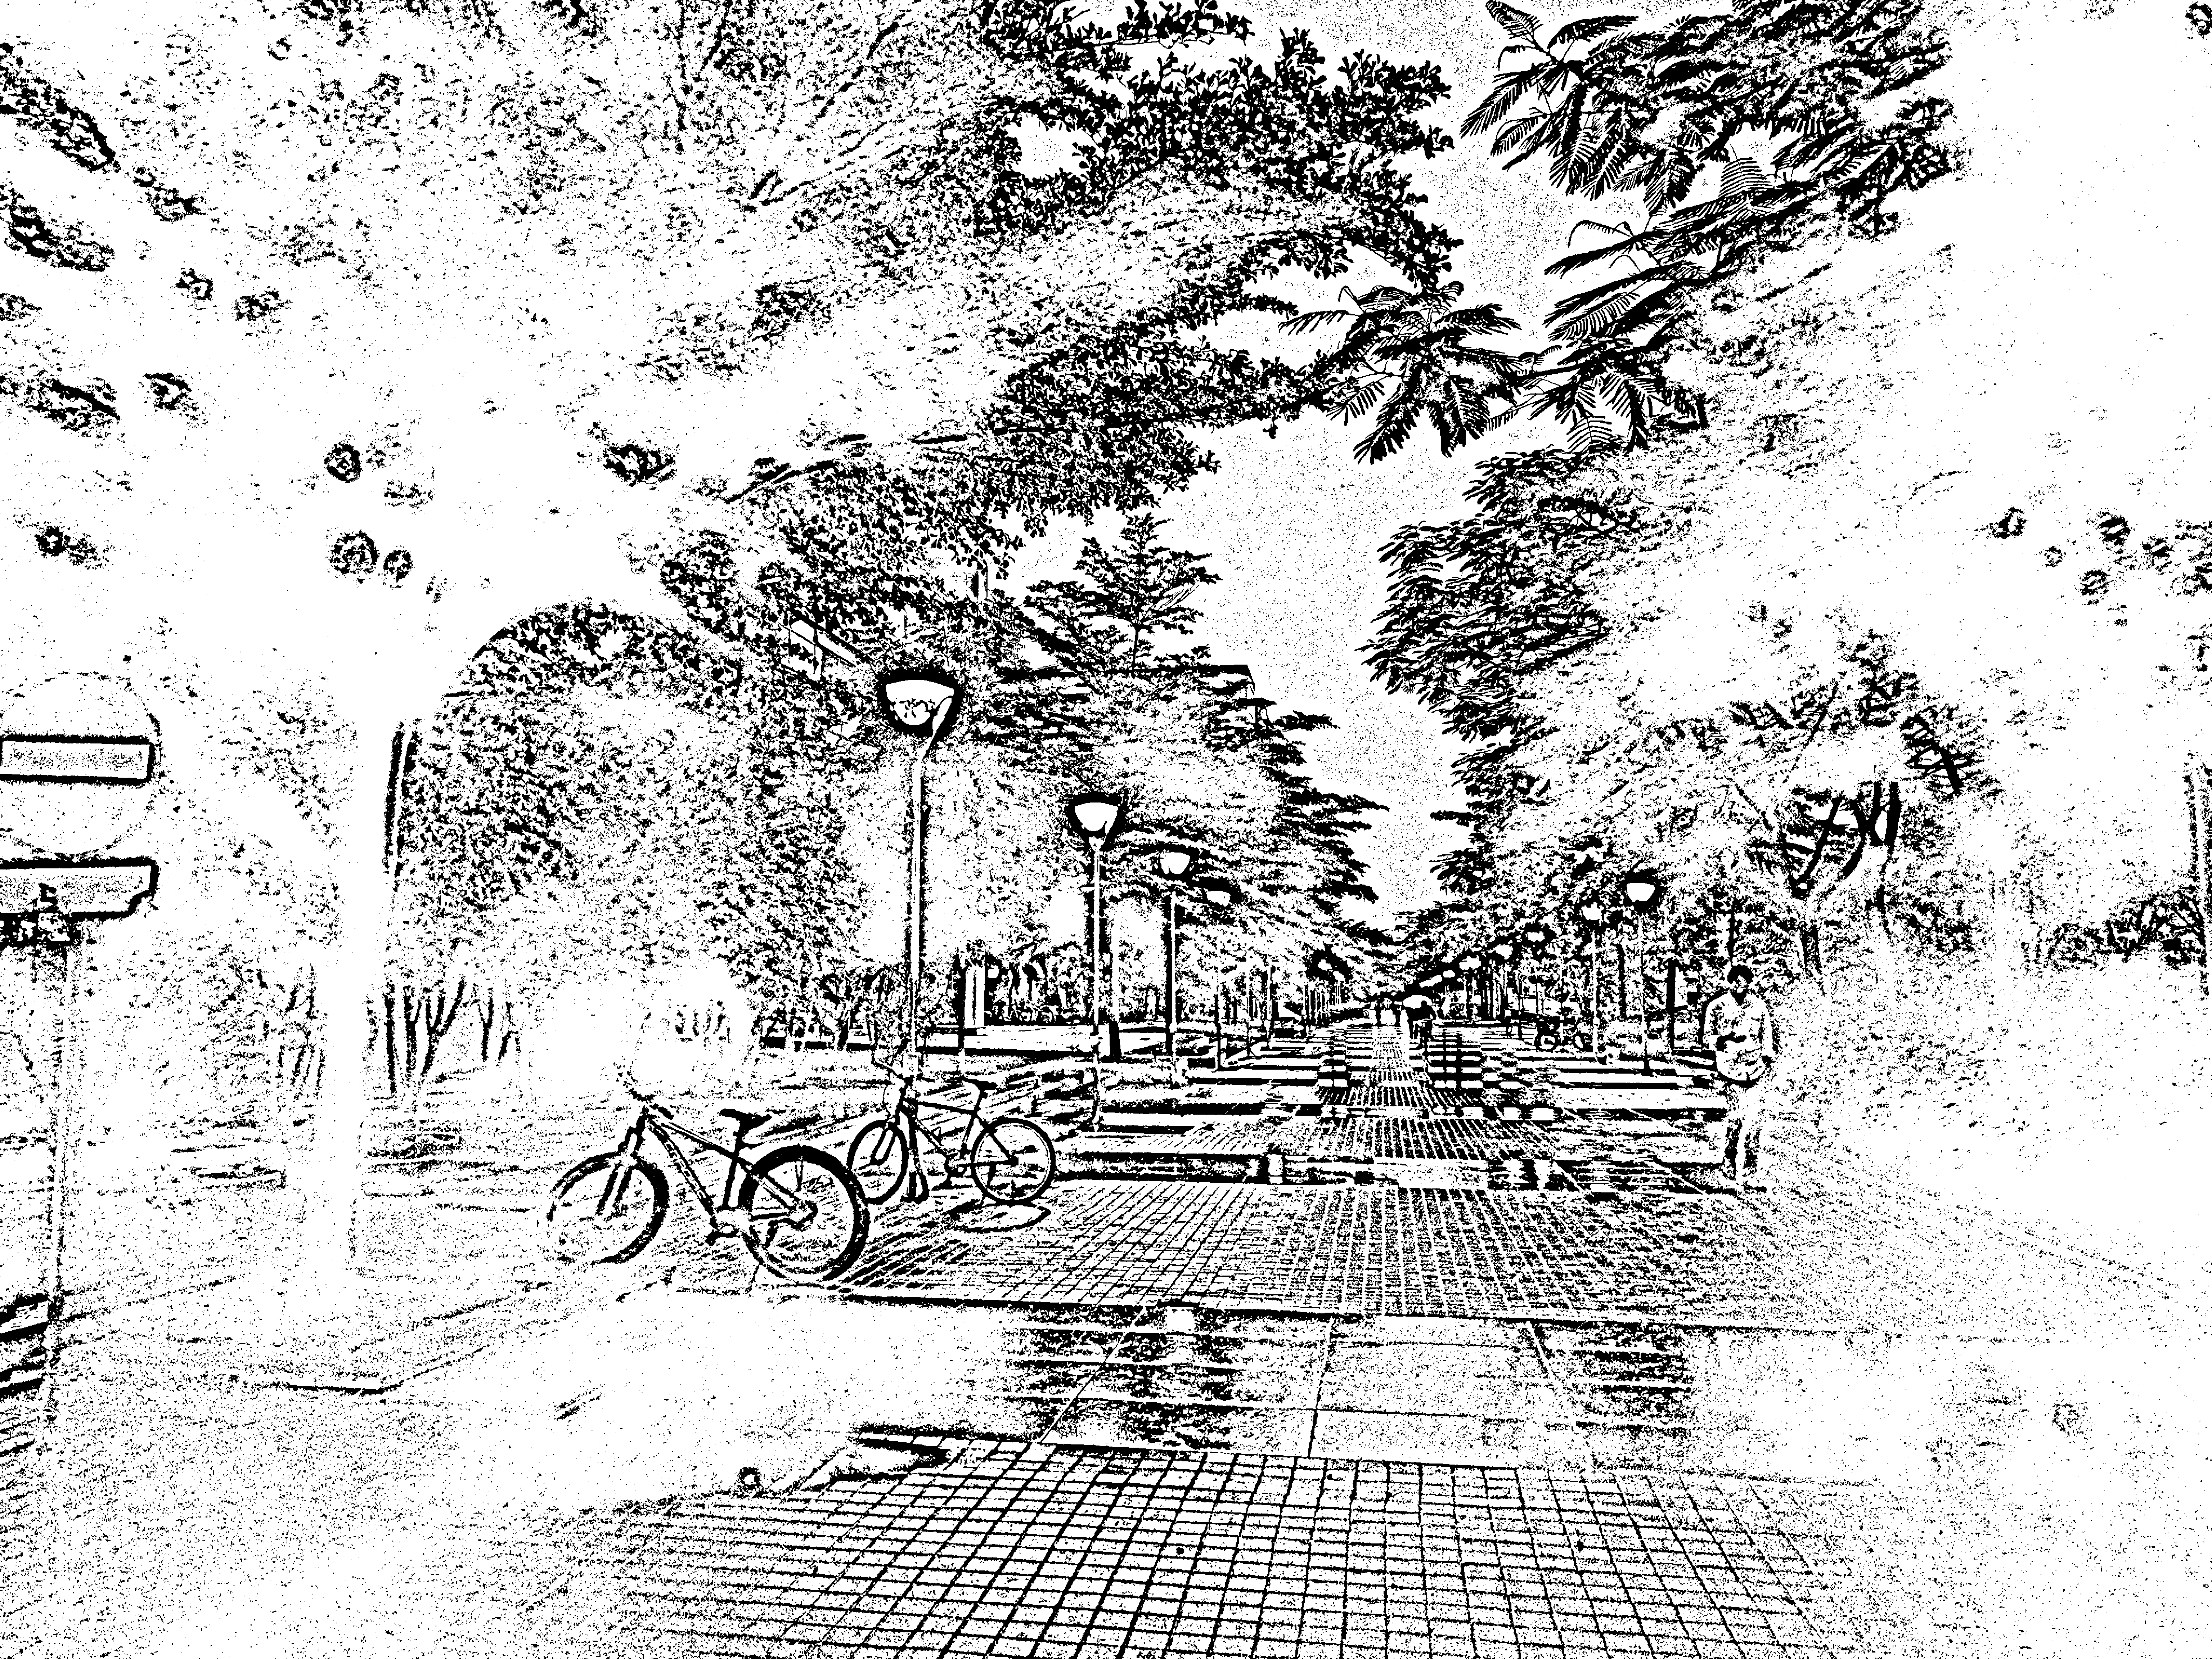
\includegraphics[width=0.5\linewidth]{figs/scenery/gaussian_localized_reference.pdf}
    \caption{Gaussian localized reference with $\sigma=10$ and $C=3$.}
    \label{fig:scenery_gaussian_localized}
\end{figure}

\begin{figure}[H]
    \centering
    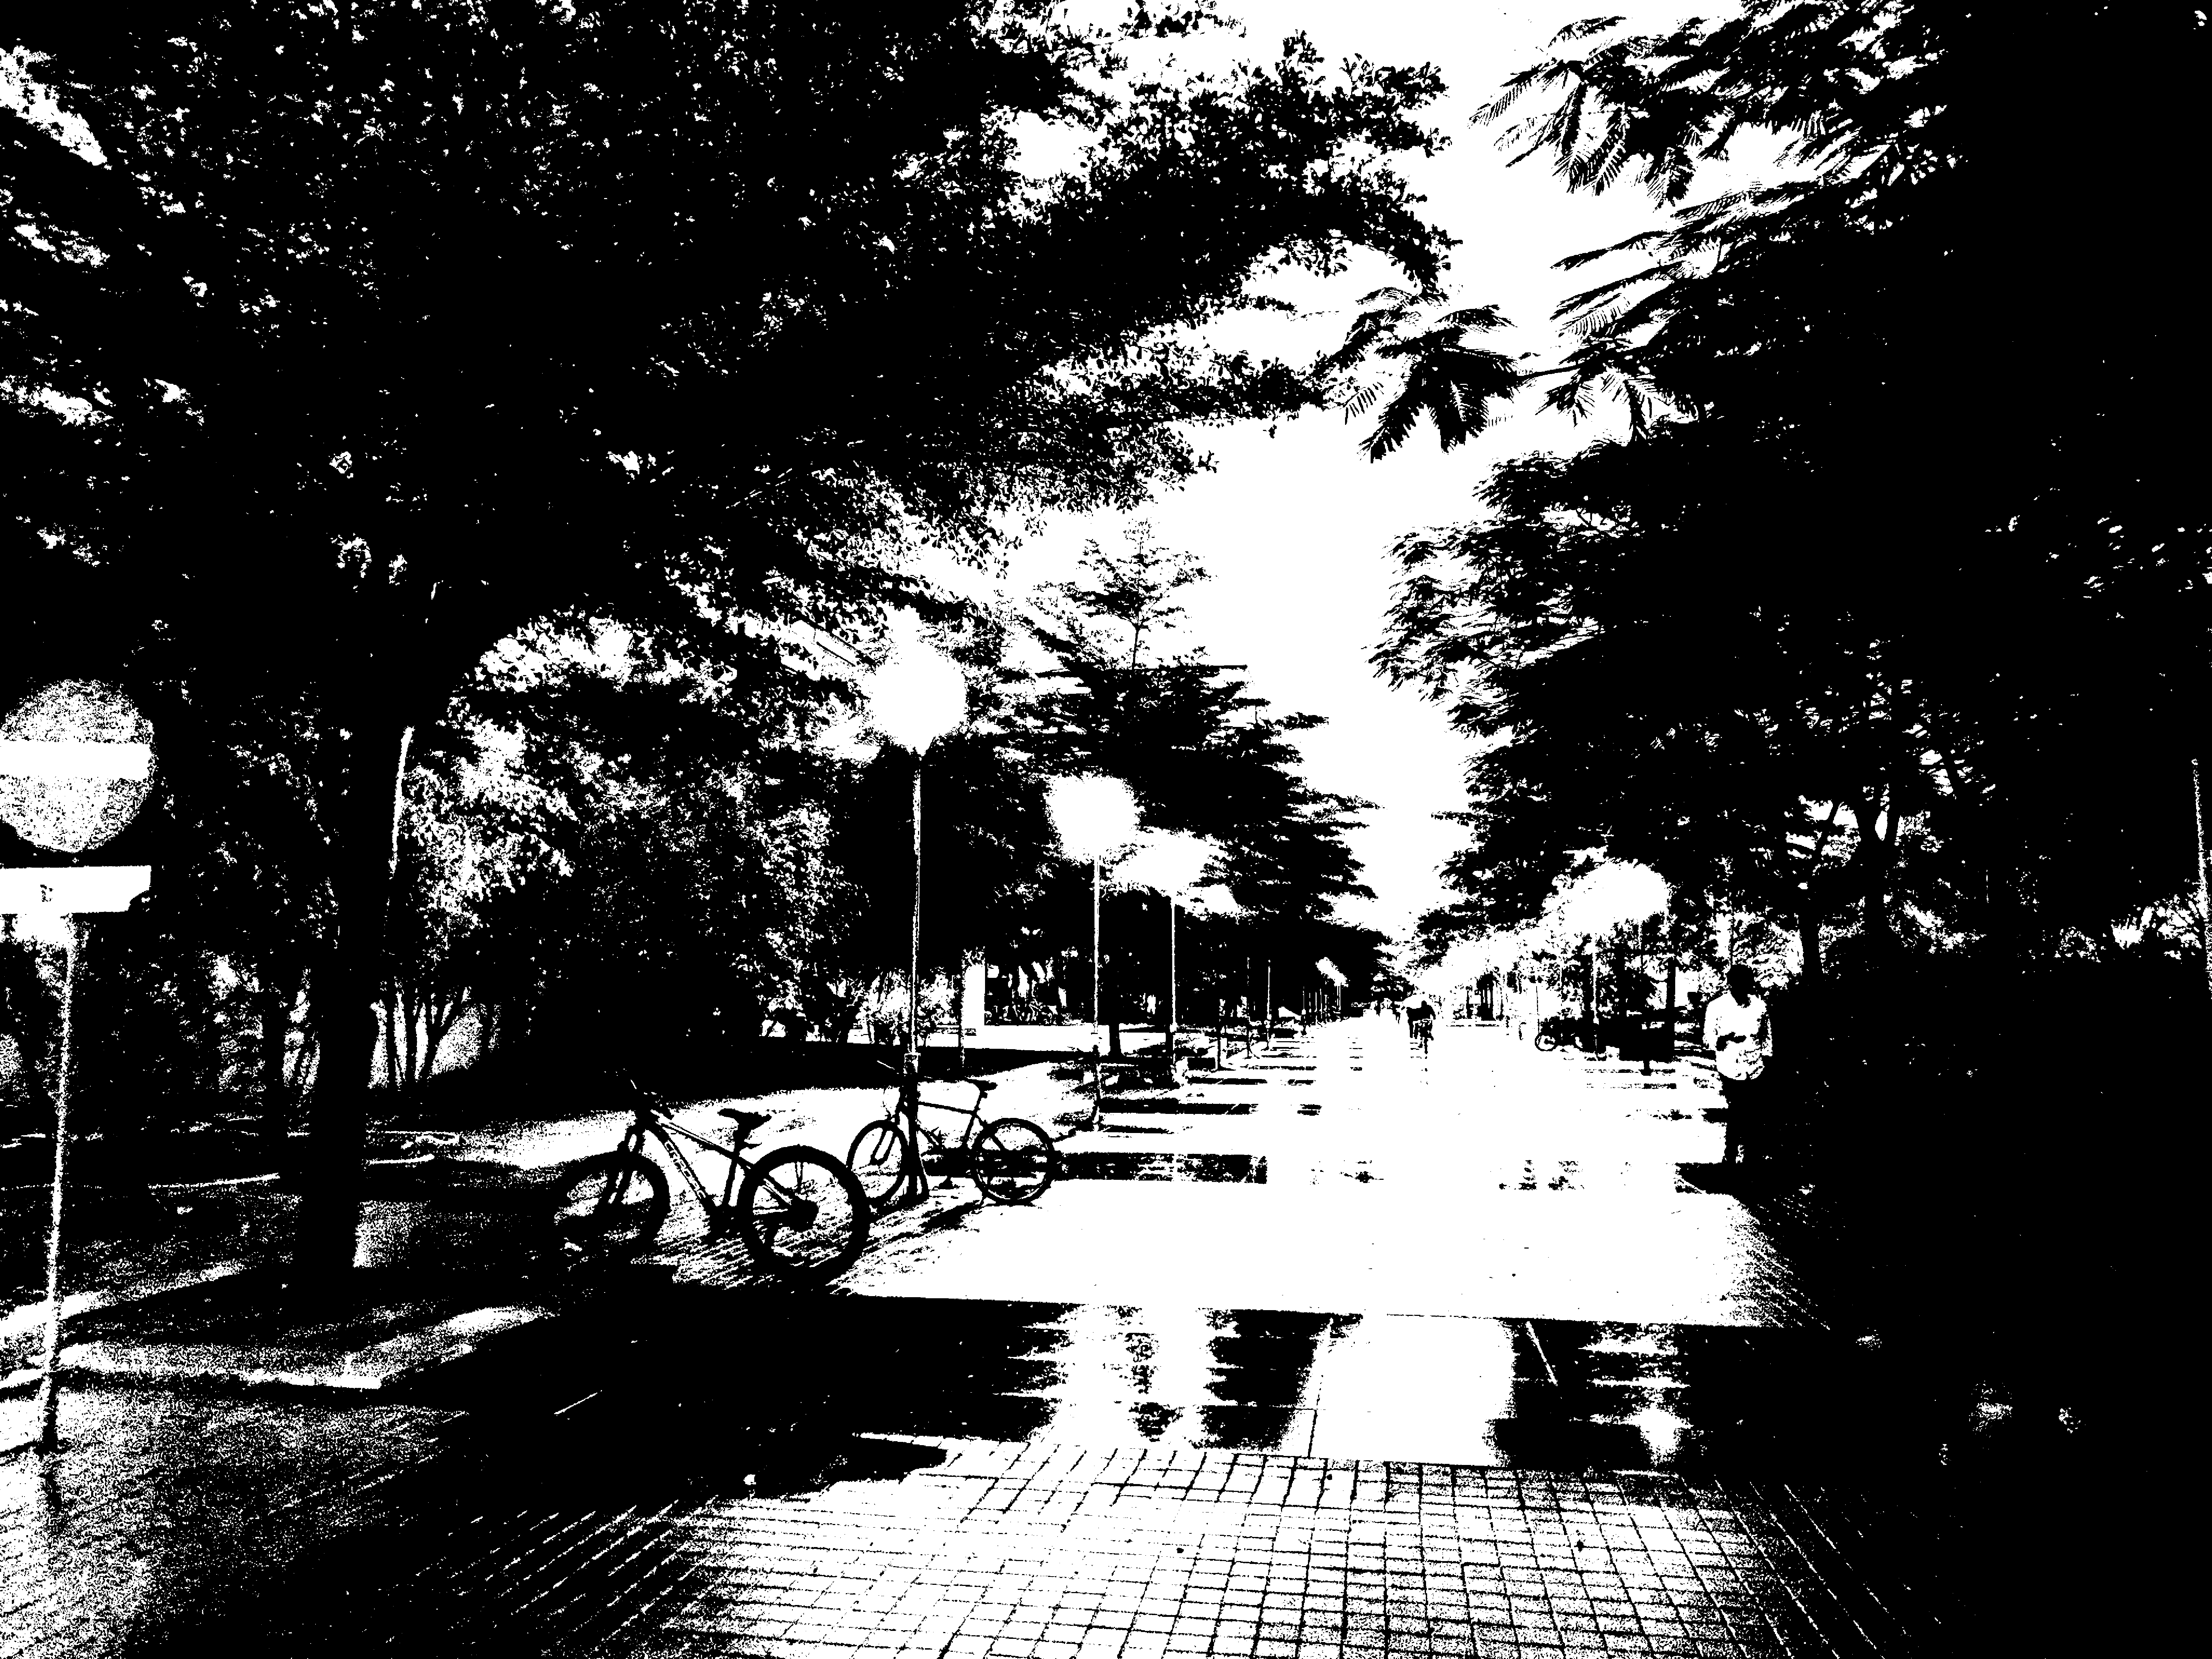
\includegraphics[width=0.5\linewidth]{figs/scenery/gaussian_wide_reference.pdf}
    \caption{Gaussian wide reference with $\sigma=1200$ and $C=3$.}
    \label{fig:scenery_gaussian_wide}
\end{figure}
\vspace*{\baselineskip}
\subsection{Testing Case 2: Jersey}

The second test case uses a jersey image. The same sequence is retained
to make the behaviour of the reference methods directly comparable.

\begin{figure}[H]
    \centering
    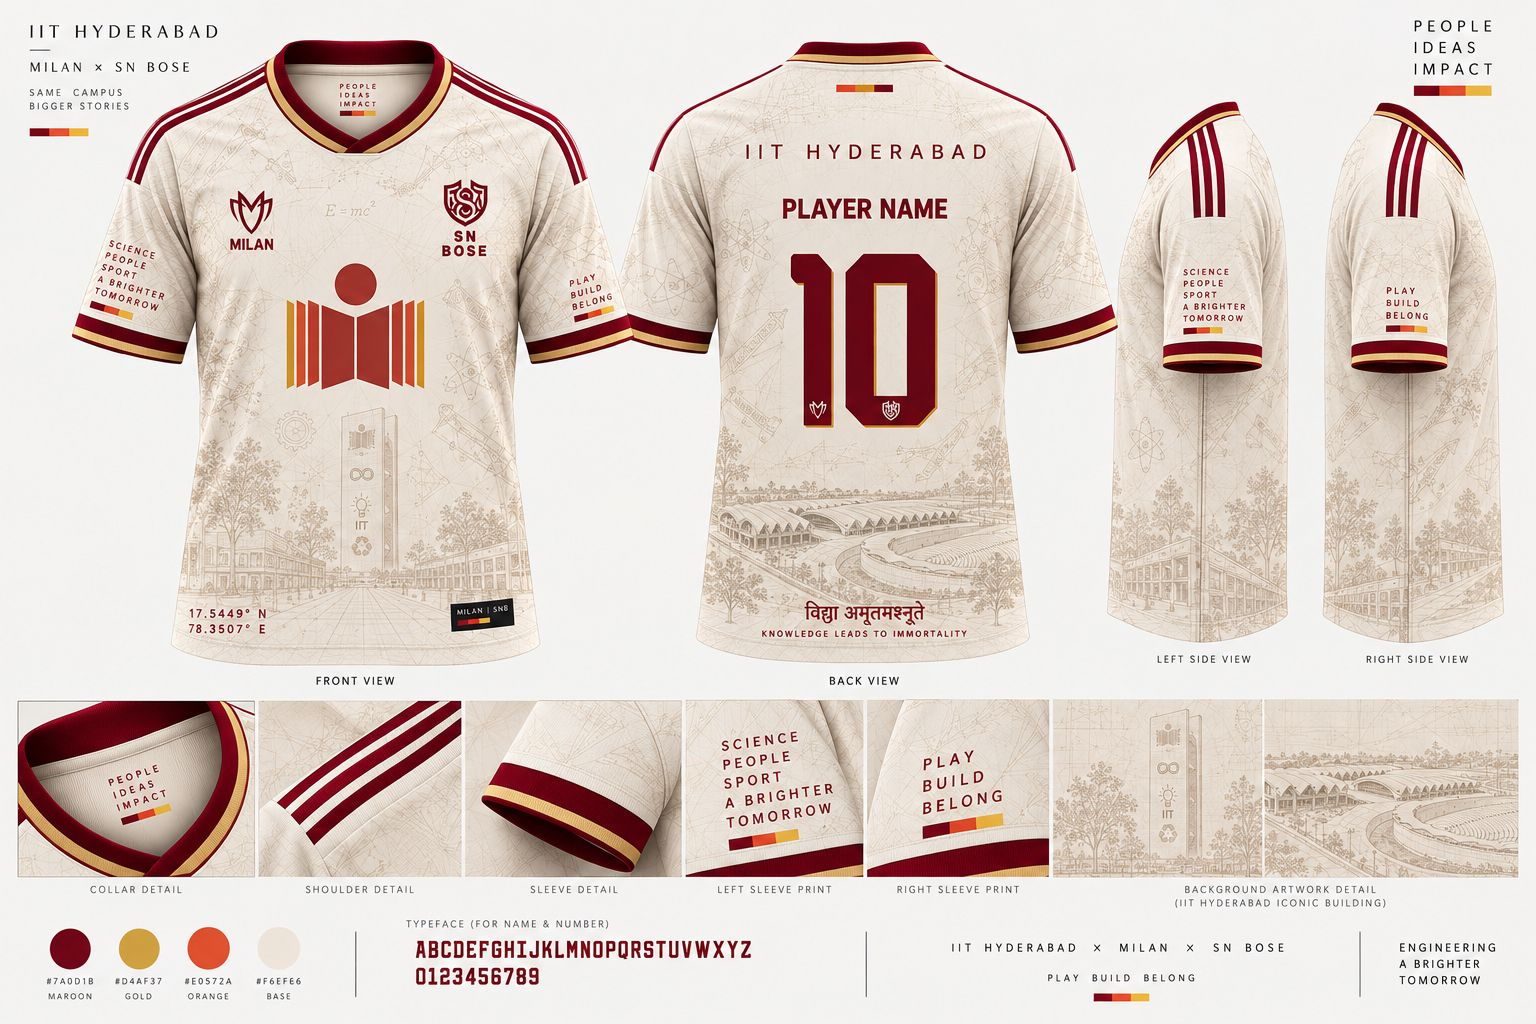
\includegraphics[width=0.5\linewidth]{figs/jersey/input.jpg}
    \caption{Input jersey image.}
    \label{fig:jersey_input}
\end{figure}

\begin{figure}[H]
    \centering
    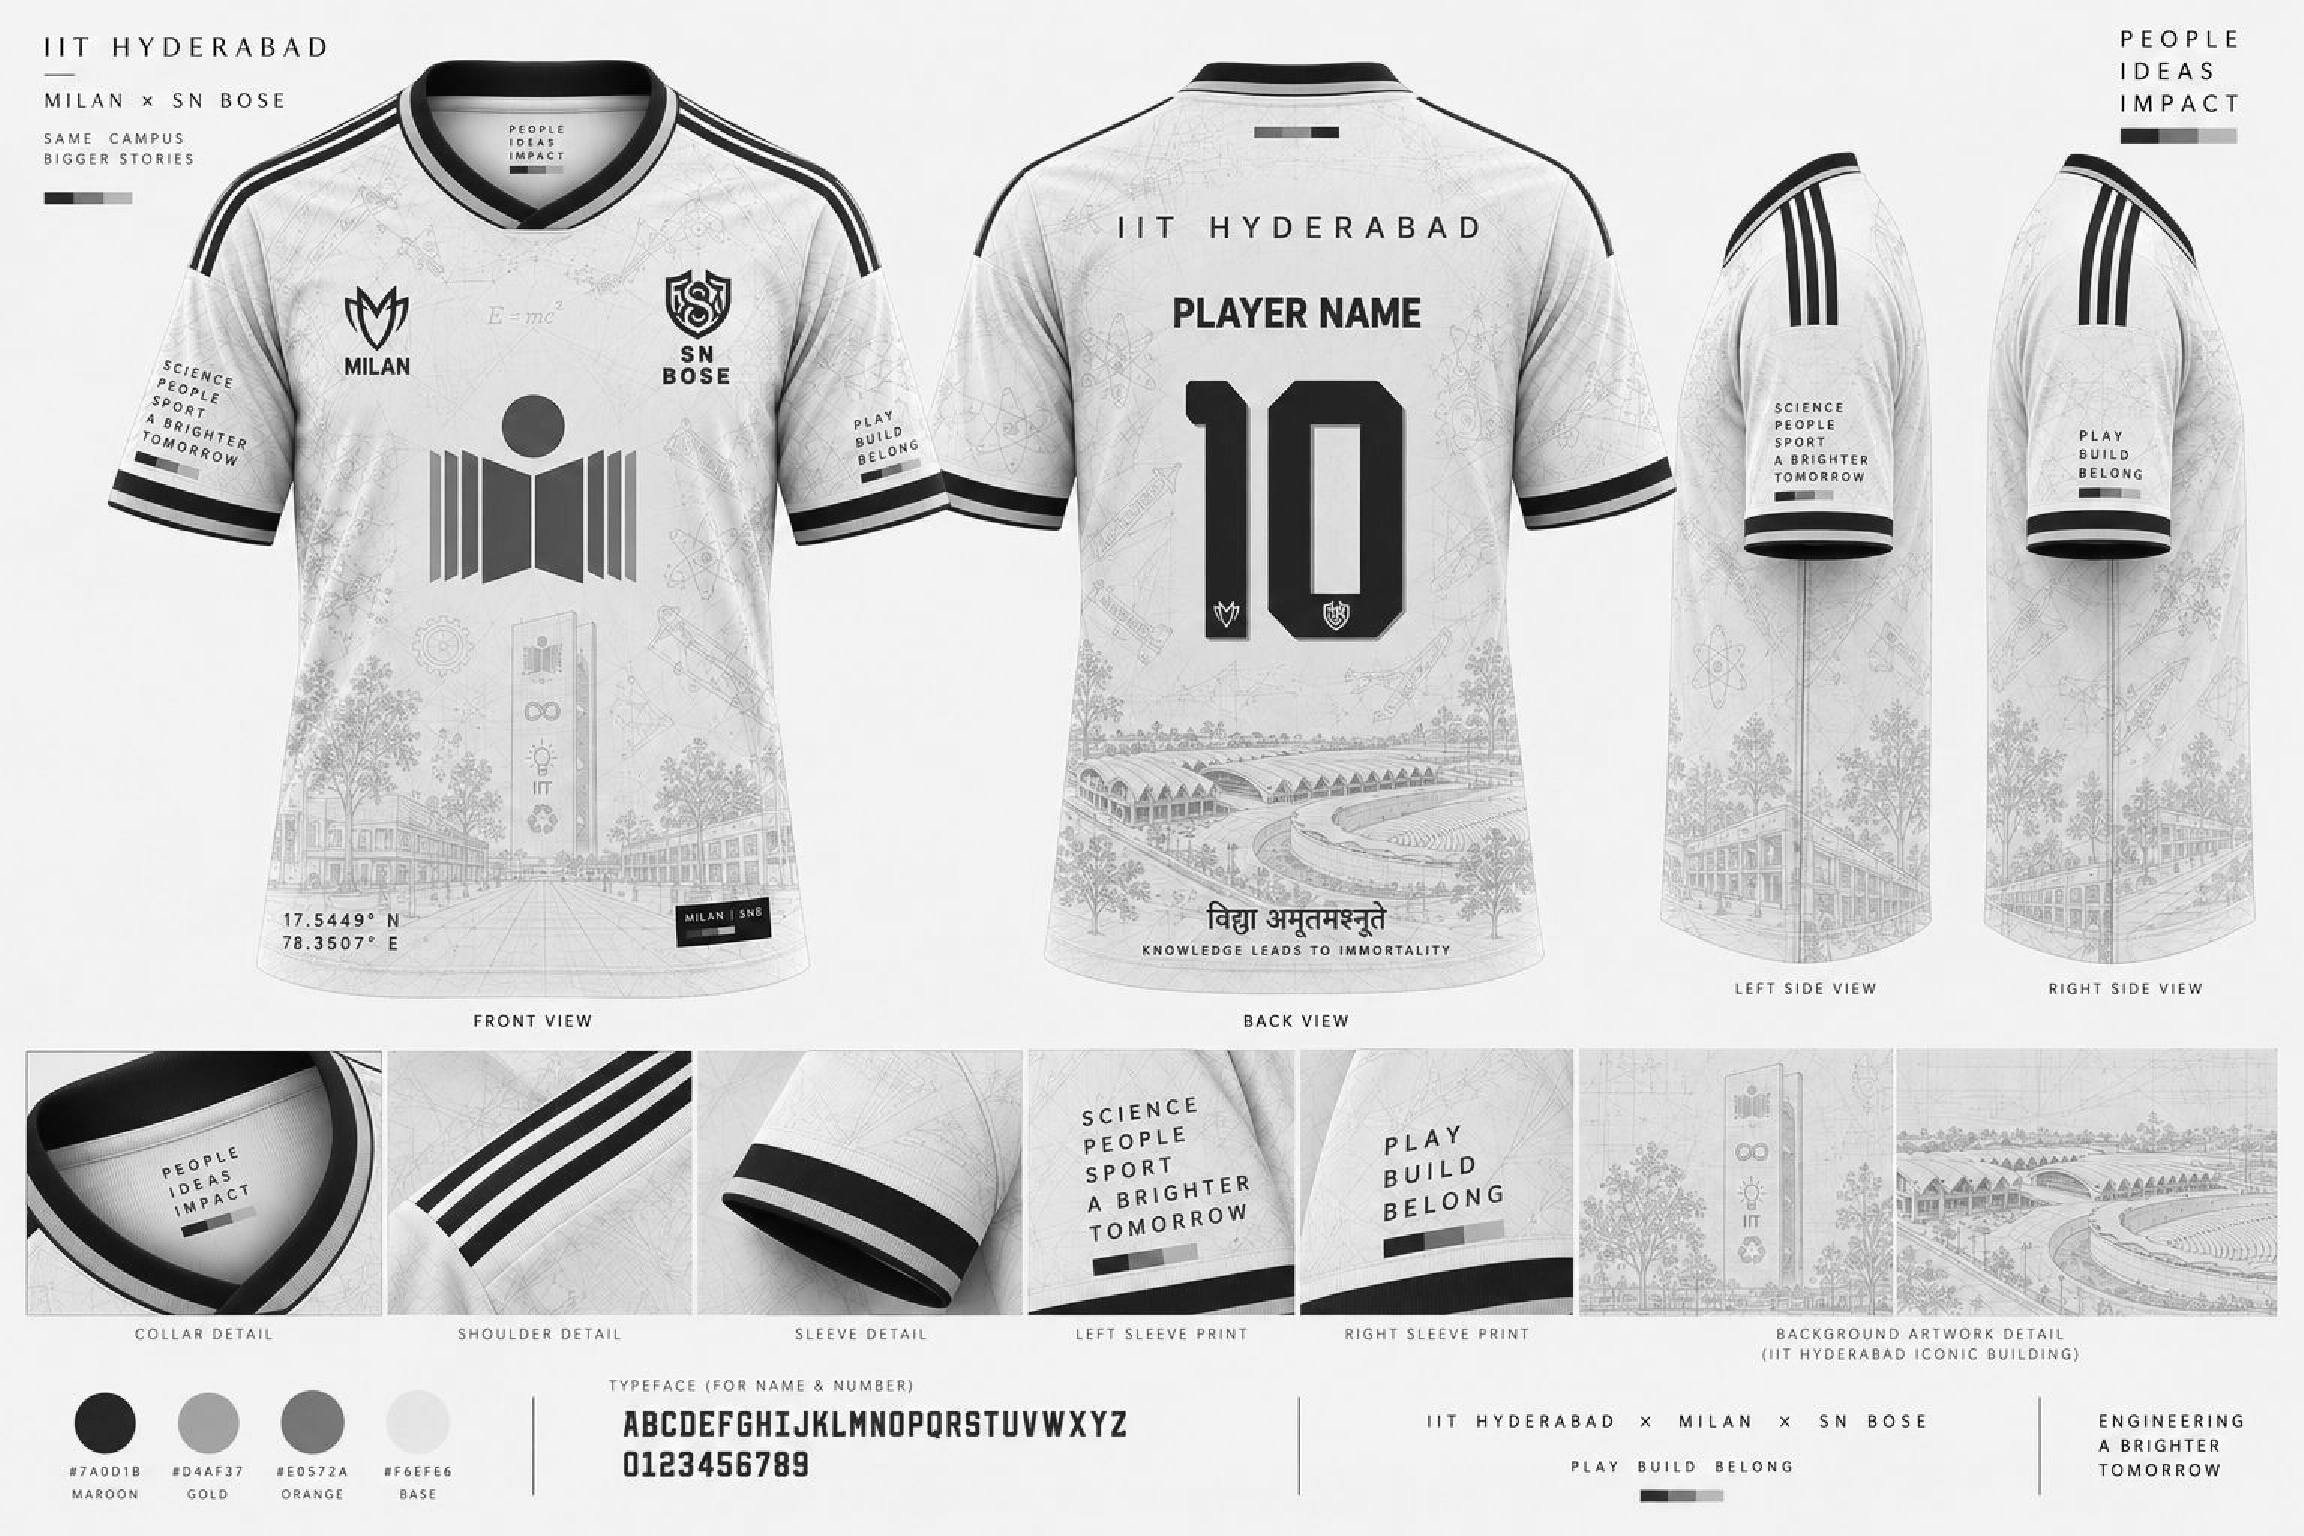
\includegraphics[width=0.5\linewidth]{figs/jersey/output_grayscale.pdf}
    \caption{Grayscale representation of the jersey image.}
    \label{fig:jersey_grayscale}
\end{figure}

\begin{figure}[H]
    \centering
    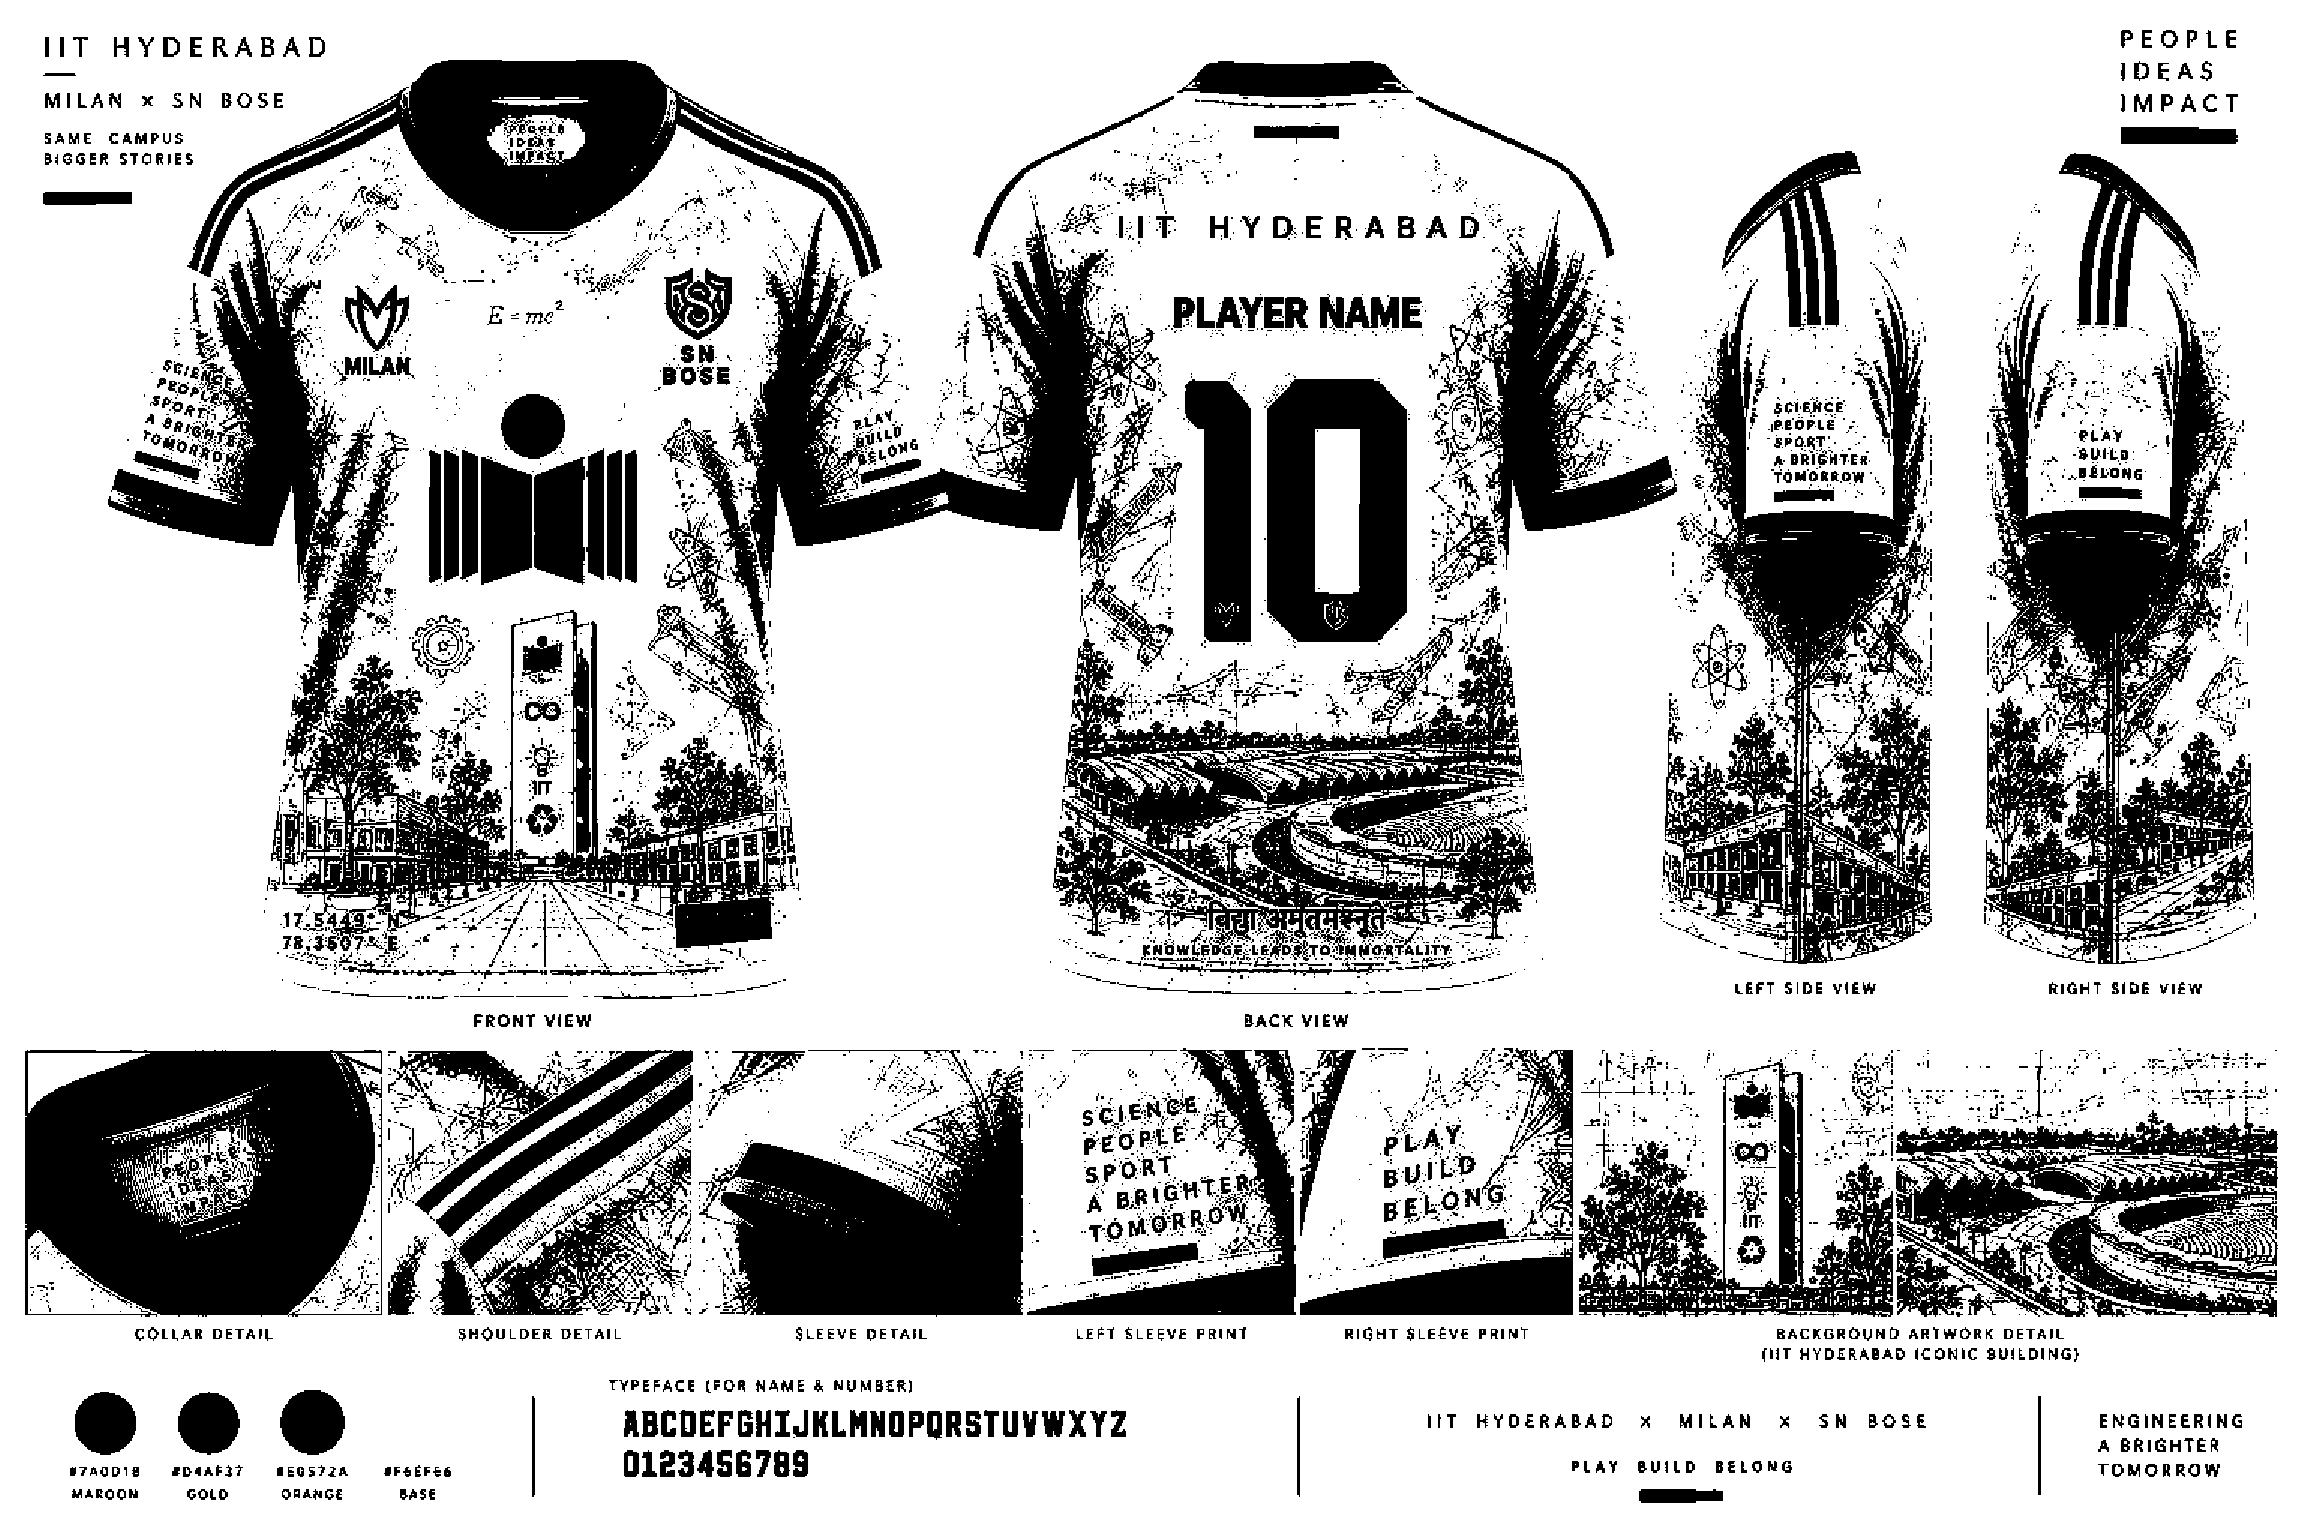
\includegraphics[width=0.5\linewidth]{figs/jersey/averaged_reference.pdf}
    \caption{Global mean adaptive thresholding of the jersey image.}
    \label{fig:jersey_adaptive}
\end{figure}

\begin{figure}[H]
    \centering
    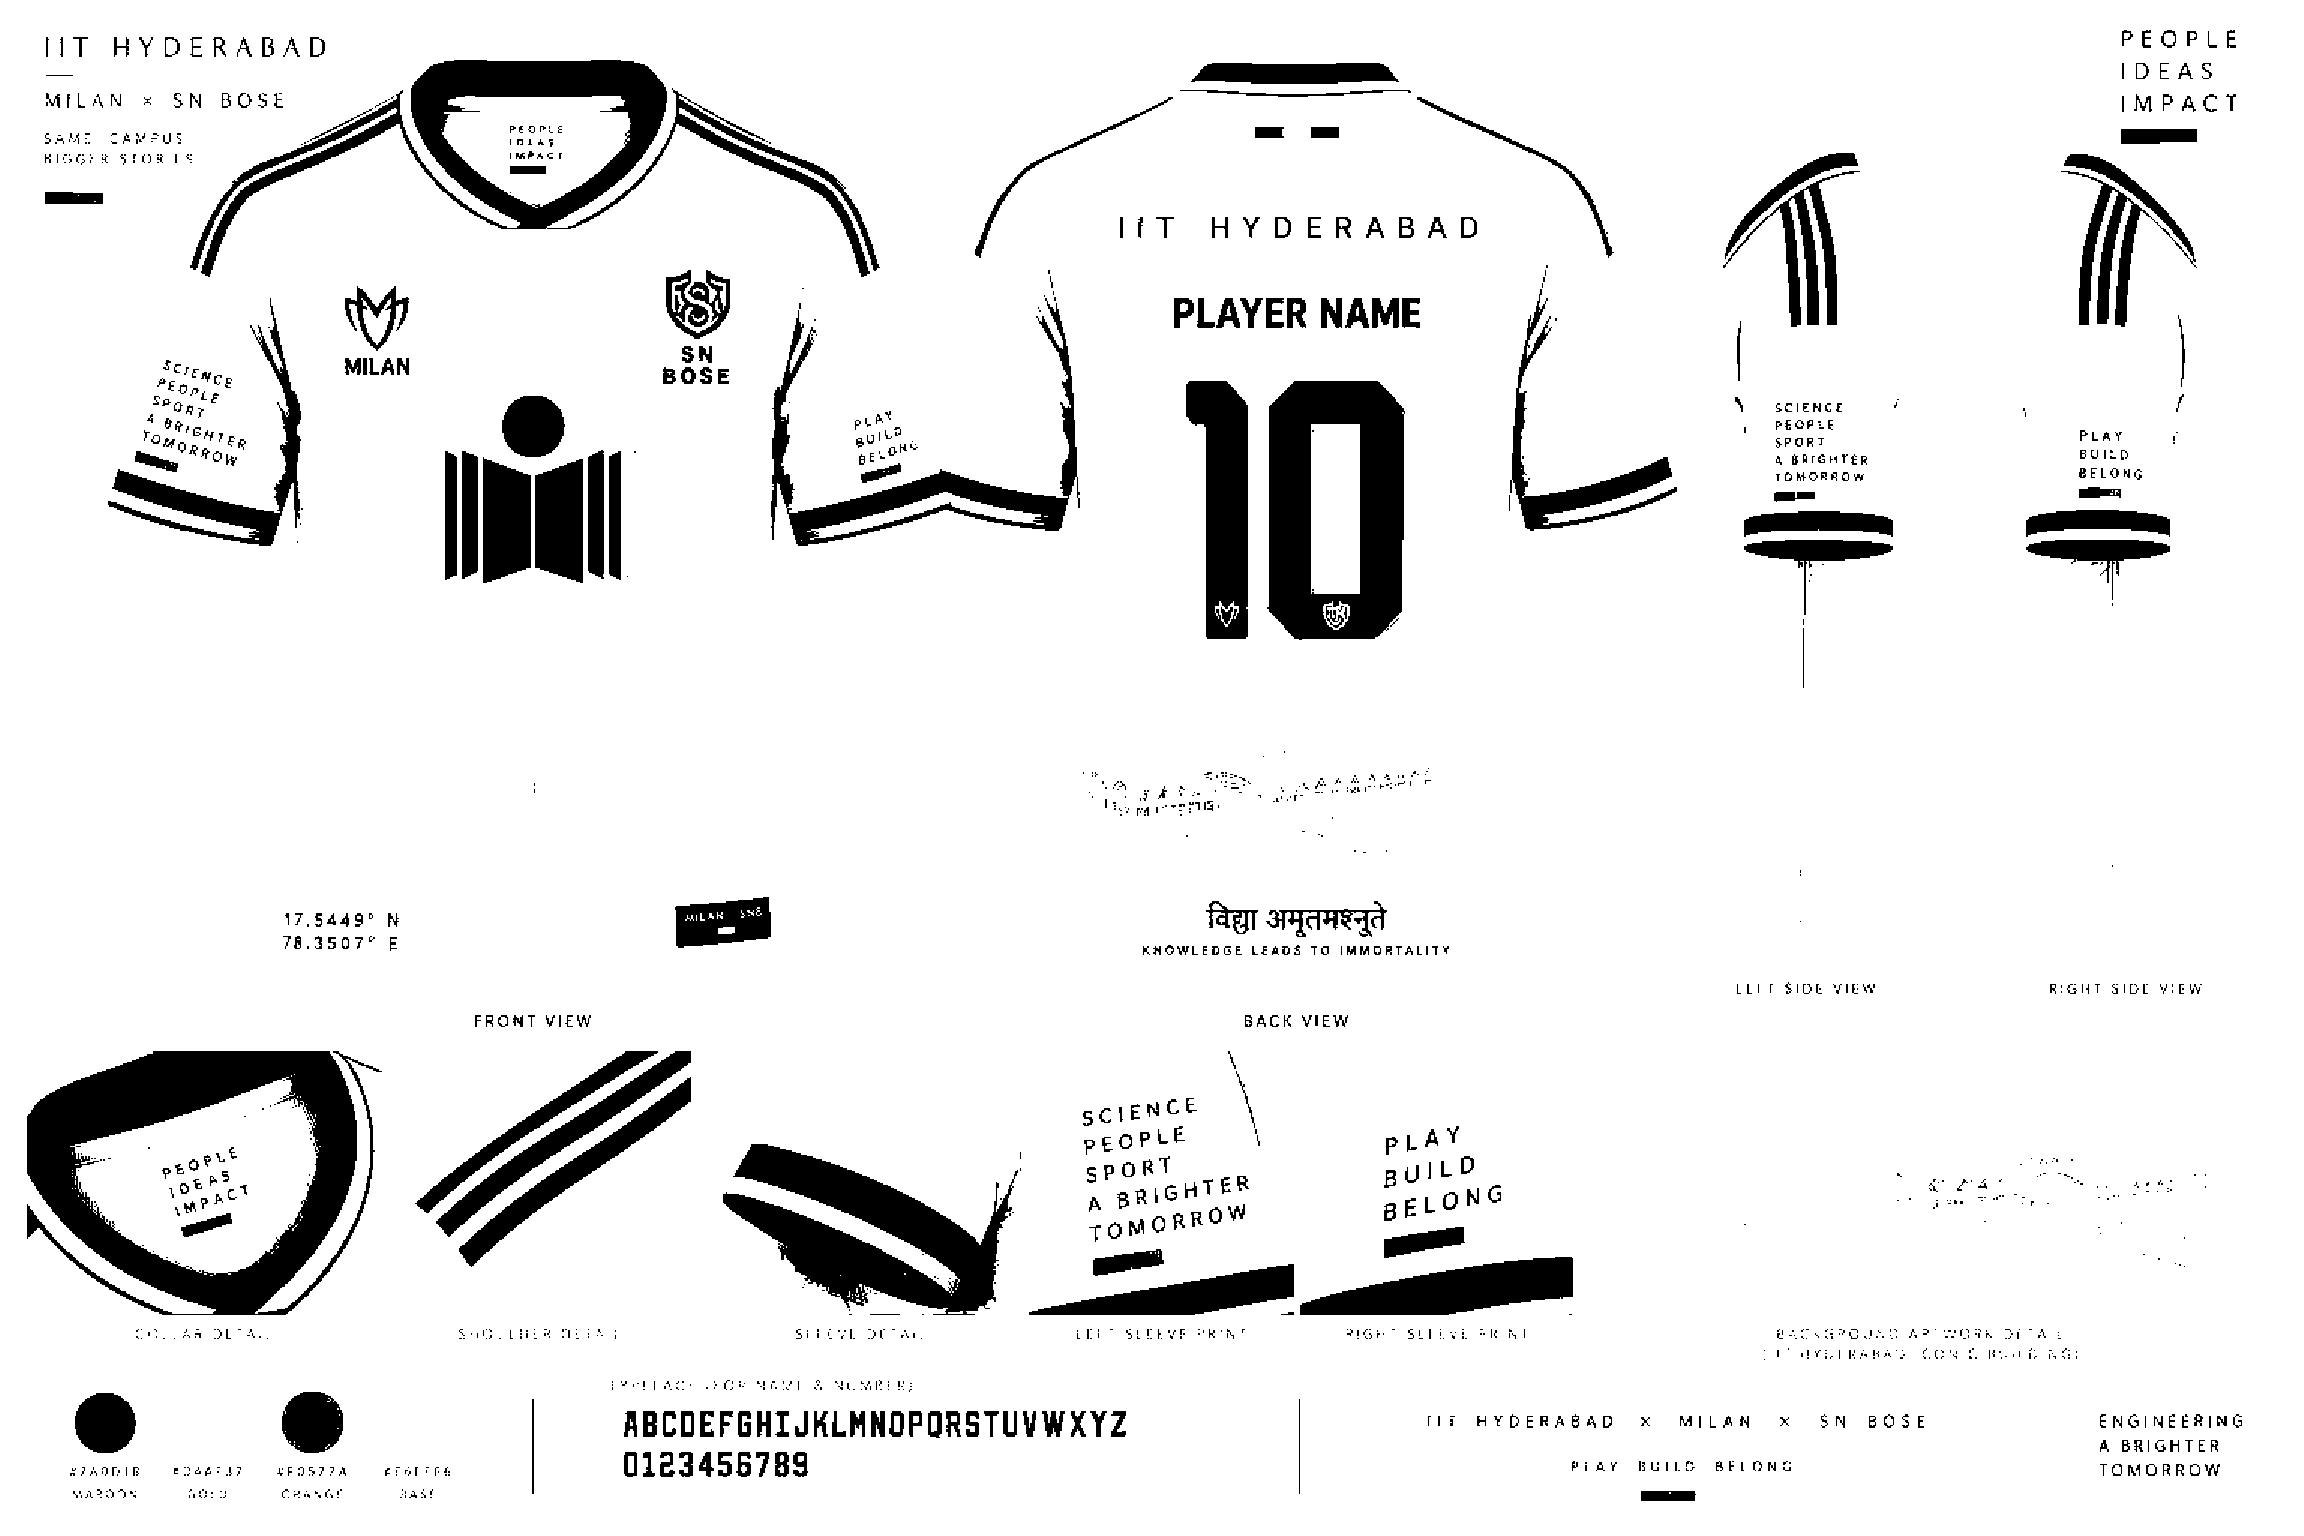
\includegraphics[width=0.5\linewidth]{figs/jersey/fixed_reference.pdf}
    \caption{Static thresholding using the fixed reference of $128$.}
    \label{fig:jersey_static}
\end{figure}

\begin{figure}[H]
    \centering
    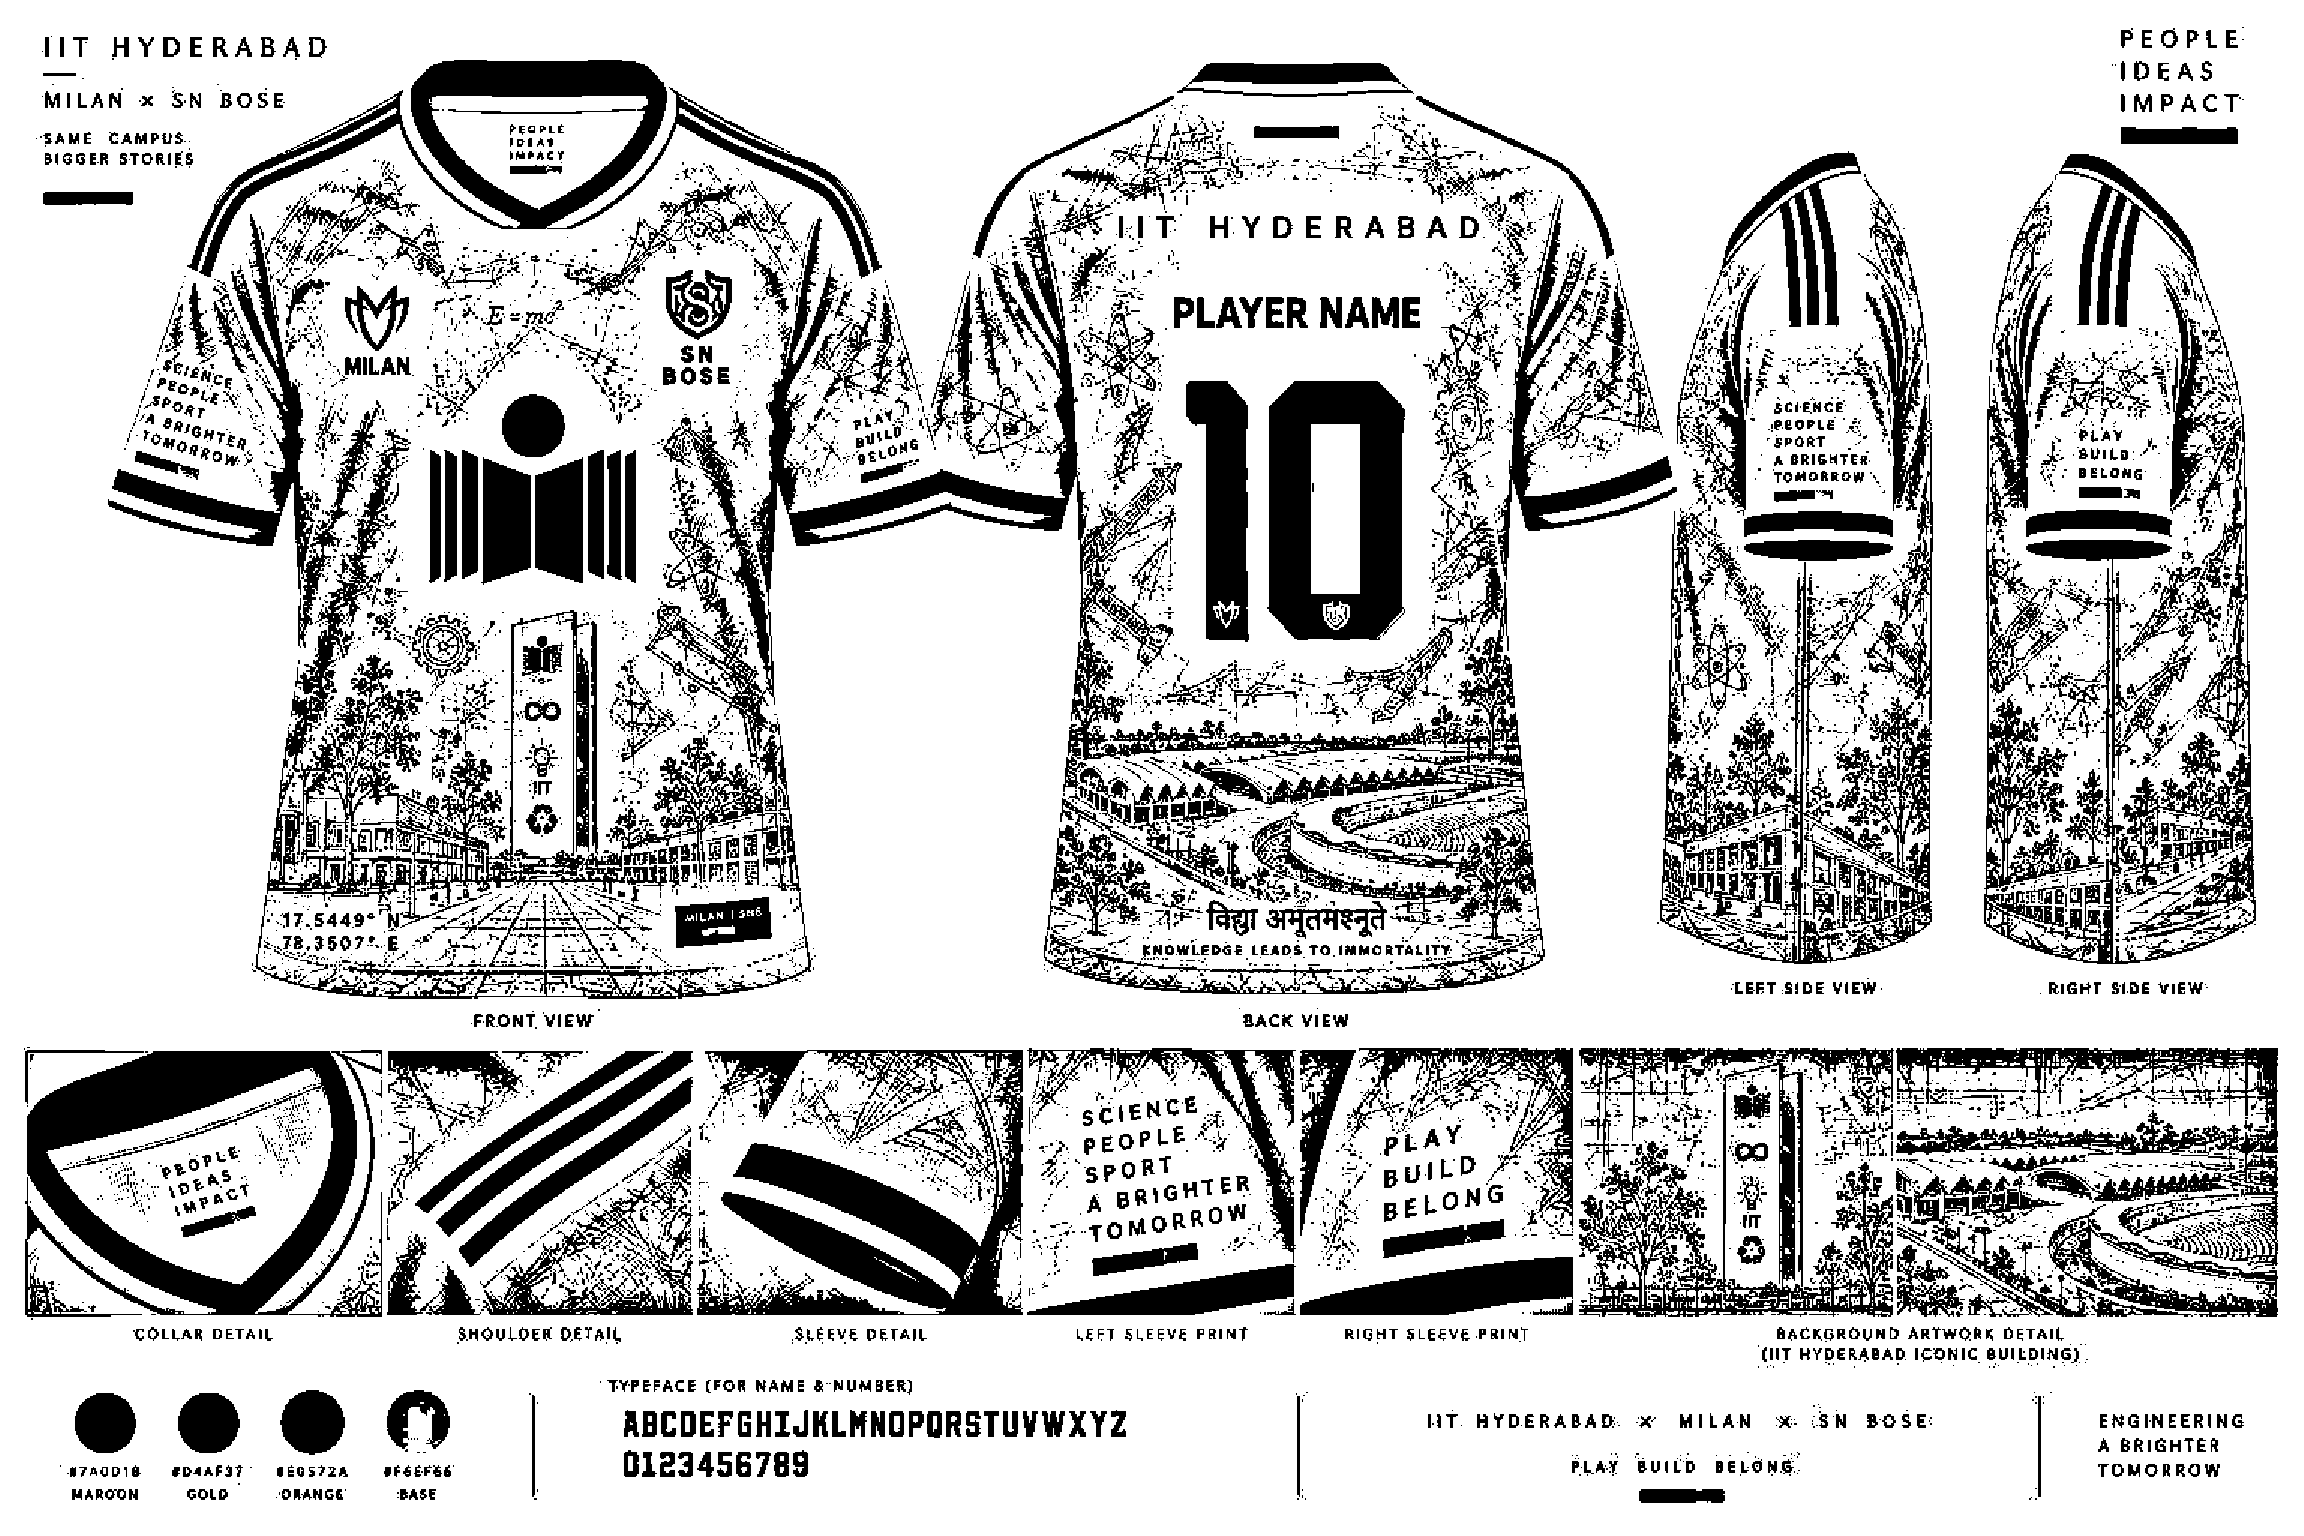
\includegraphics[width=0.5\linewidth]{figs/jersey/gaussian_localized_reference.pdf}
    \caption{Gaussian localized reference with $\sigma=10$ and $C=3$.}
    \label{fig:jersey_gaussian_localized}
\end{figure}

\begin{figure}[H]
    \centering
    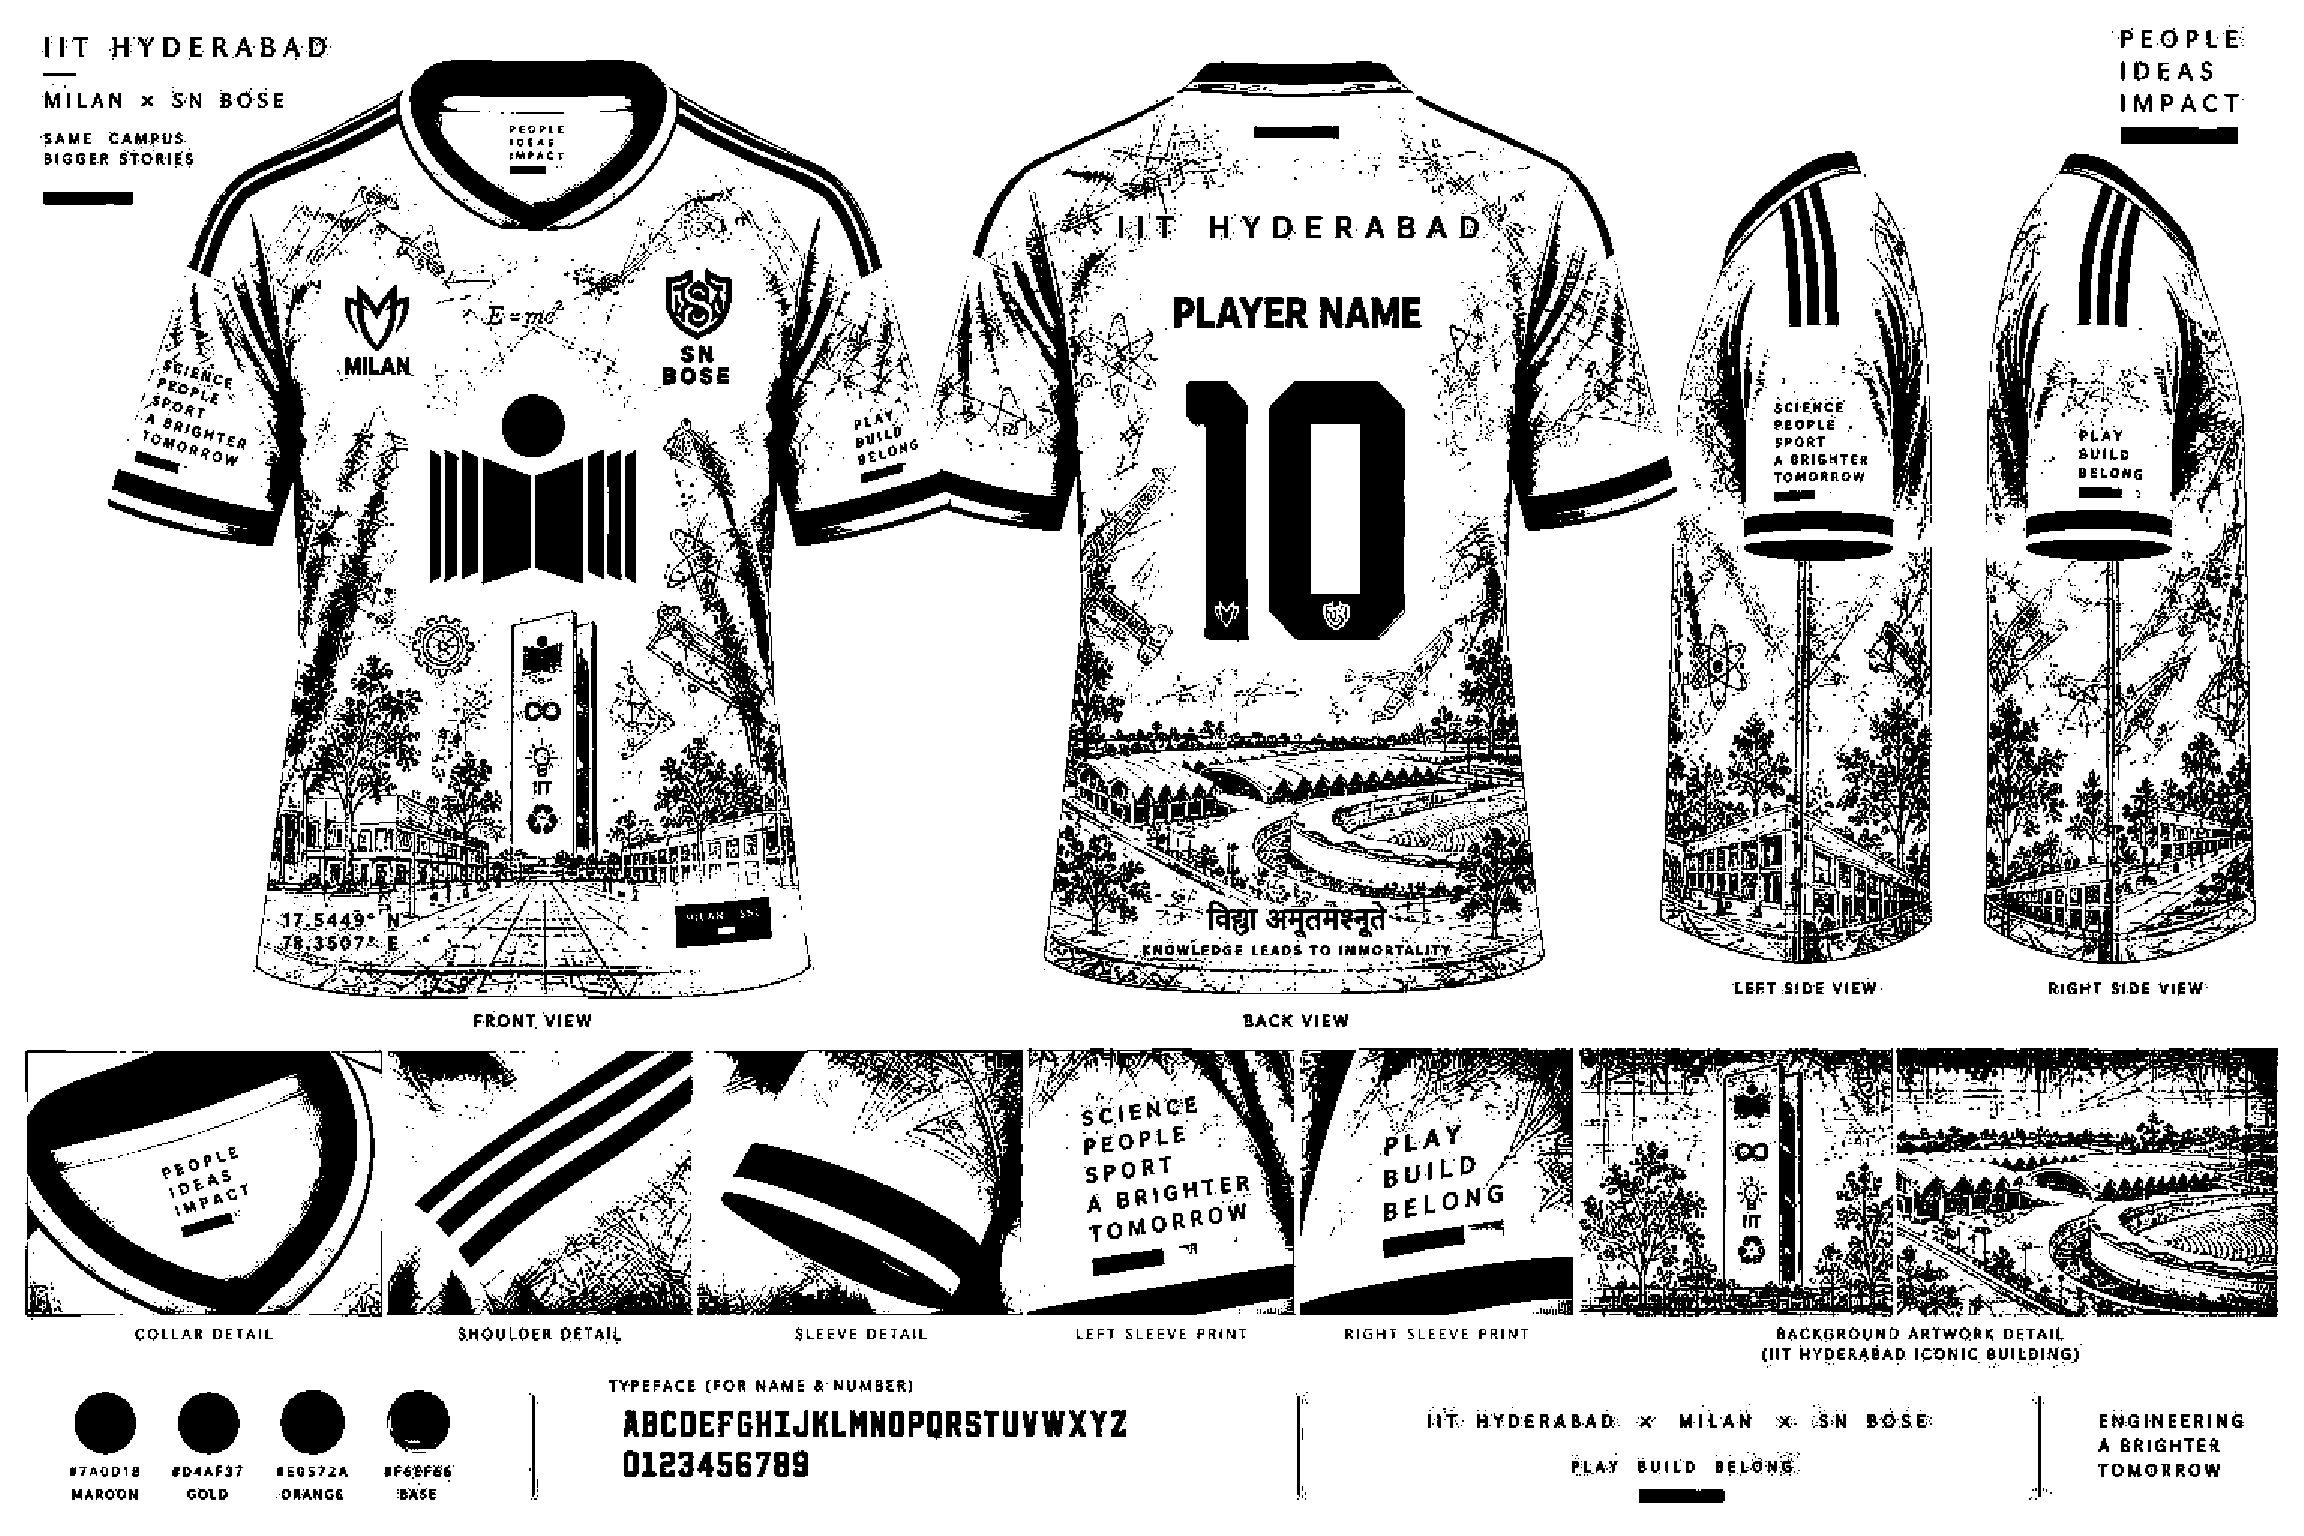
\includegraphics[width=0.5\linewidth]{figs/jersey/gaussian_wide_reference.pdf}
    \caption{Gaussian wide reference with $\sigma=20$ and $C=3$.}
    \label{fig:jersey_gaussian_wide}
\end{figure}
\vspace*{\baselineskip}
\subsection{Program File}

The complete Python code used to generate the grayscale and
black-and-white outputs is:

\begin{lstlisting}[frame=single, basicstyle=\rmfamily, escapeinside={(*@}{@*)}]
(*@\makebox[\dimexpr\linewidth-2\fboxsep-2\fboxrule\relax][c]{codes/image.py}@*)
\end{lstlisting}
